\section{Results}
\label{fourthchapter}

\label{sec:res_intro}
This chapter presents the results of the global warming potential (GWP) optimisation across the four occupancy scenarios and the practical span range of 3--10\,m. Five floor systems are compared: the composite steel--concrete slab developed in this work, two reinforced concrete baselines (a solid flat slab, \texttt{RC flat}, and a ribbed slab, \texttt{RC ribbed}), and two timber baselines (a solid rectangular slab, \texttt{timber flat}, and a ribbed slab, \texttt{timber ribbed}) inherited from the pre-existing framework.

Two points on the scope of the comparison apply throughout. First, only the composite slab and the RC flat slab are analysed as continuous members; the RC ribbed and timber systems were not extended to continuous spans within the pre-existing framework. In the two-- and three--span figures that follow, these systems are therefore shown at their single--span values as reference baselines and do not represent re-analysed continuous designs. Second, the office occupancy is treated as the principal scenario and is reported in full (Section~\ref{sec:res_office}); the residential, retail, and industrial scenarios are reported in condensed form (Section~\ref{sec:res_other}), with the complete per--span tables, breakdowns, and supporting figures collected in Appendix~\ref{app:results_figures}.

For each system, span, and span configuration, the optimiser returns the minimum--GWP cross--section that satisfies all applicable design checks. This combined--criterion result is referred to as the \emph{envelope} (ENV) optimum and forms the basis of all GWP comparisons. Where it is informative to show why a particular limit state governs, the results of the single--criterion runs (ULS, SLS, and fire considered in isolation) are used. Total GWP (\(\mathrm{GWP}_\mathrm{tot}\)) comprises the structural slab contribution (\(\mathrm{GWP}_\mathrm{struct}\)) plus the fixed non--structural floor build--up; all values are reported per square metre of floor area.

%==============================================================================
\subsection{Office scenario}
\label{sec:res_office}
%==============================================================================
The office scenario uses an imposed load of 2.5 + 0.50\,kN/m$^2$ with a raised--access--floor build--up (Section~\ref{sec:floor_buildup}). It is presented here in full; the other occupancies follow the same structure in condensed form.

%------------------------------------------------------------------
\subsubsection{GWP comparison across floor systems}
\label{sec:res_office_gwp}
%------------------------------------------------------------------
Figure~\ref{fig:office_gwp} compares the total GWP of the five systems against span for the single--, two--, and three--span configurations. The optimal composite cross--sections for all three configurations are listed in Table~\ref{tab:office_optima}.
 
\begin{figure}[h!]
    \centering
    \begin{subfigure}{\textwidth}
        \centering
        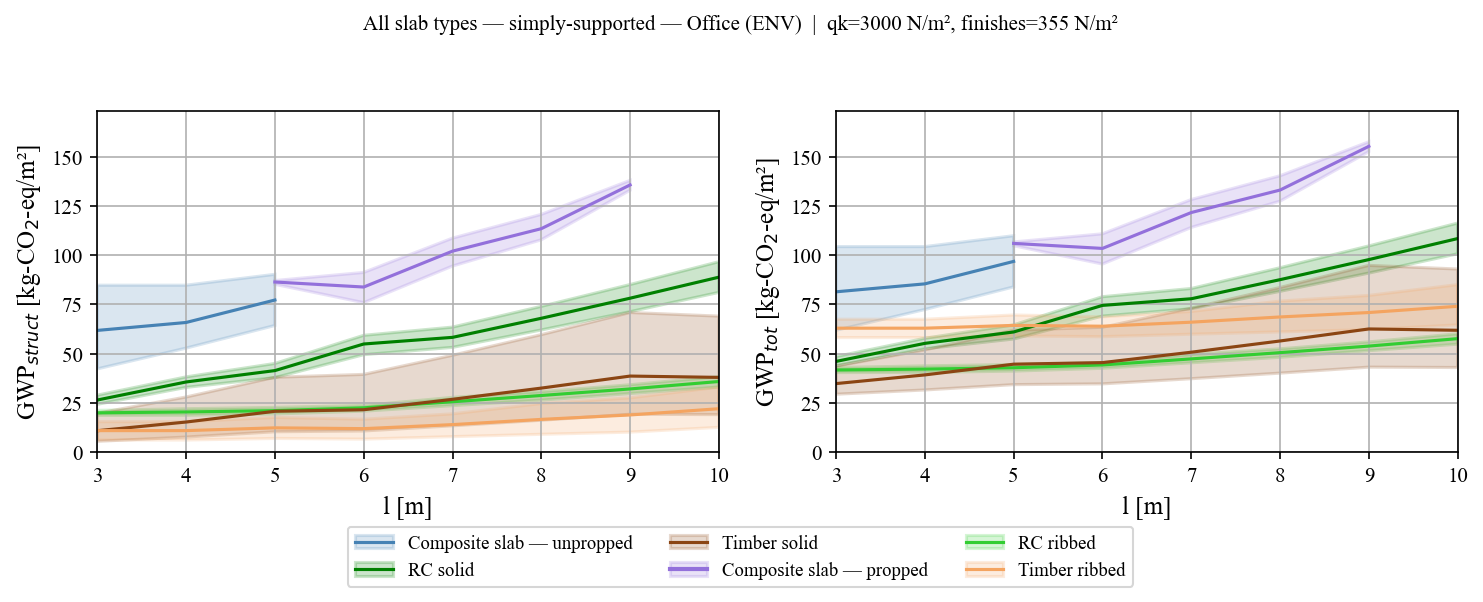
\includegraphics[width=\textwidth]{figures/office/ENV/plot_office_1span_ENV_gwp.png}
        \caption{Single span}
        \label{fig:office_gwp_1span}
    \end{subfigure}\\[4pt]
    \begin{subfigure}{\textwidth}
        \centering
        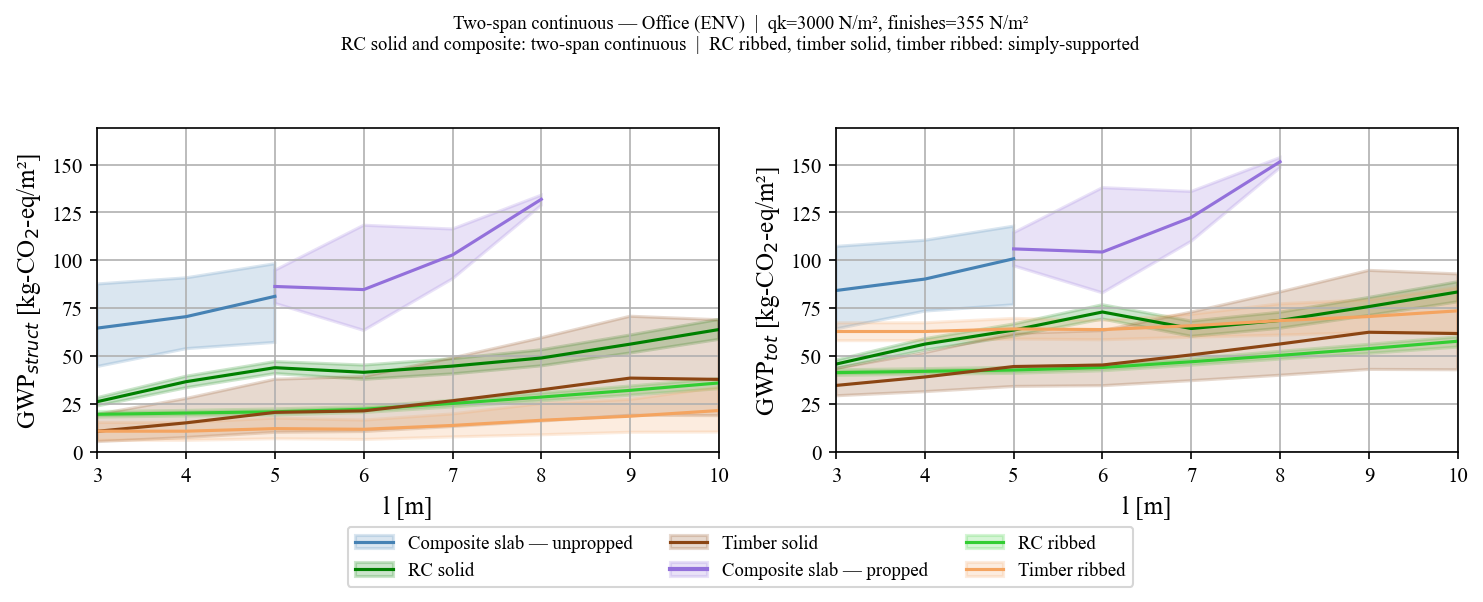
\includegraphics[width=\textwidth]{figures/office/ENV/plot_office_2span_ENV_gwp.png}
        \caption{Two--span continuous}
        \label{fig:office_gwp_2span}
    \end{subfigure}\\[4pt]
    \begin{subfigure}{\textwidth}
        \centering
        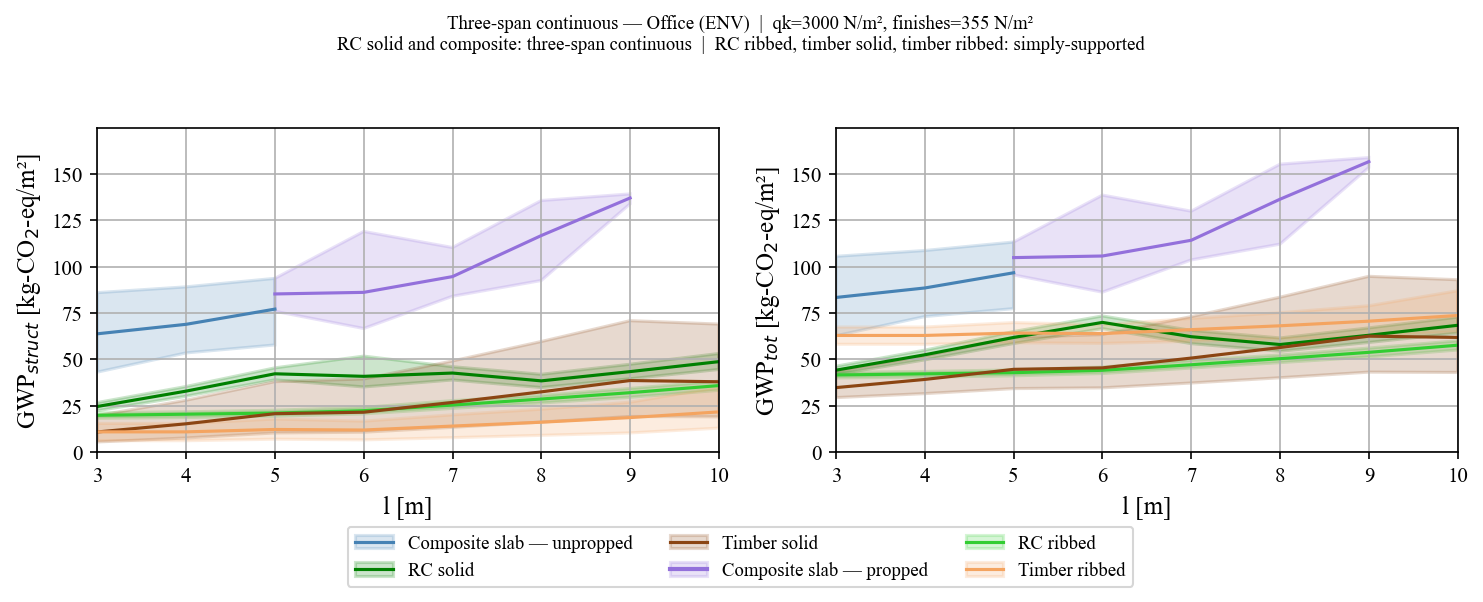
\includegraphics[width=\textwidth]{figures/office/ENV/plot_office_3span_ENV_gwp.png}
        \caption{Three--span continuous}
        \label{fig:office_gwp_3span}
    \end{subfigure}
    \caption[Office total GWP versus span]{Office scenario: total GWP per unit floor area versus span for all five floor systems, in the single--, two--, and three--span configurations.}
    \label{fig:office_gwp}
\end{figure}

The dominant result is unambiguous and holds across every span and span configuration: \textbf{the composite slab has the highest total GWP of the five systems compared}. For the single--span office case, the composite optimum rises from 67.6\,kg\,CO$_2$eq/m$^2$ at 3\,m to 152.5\,kg\,CO$_2$eq/m$^2$ at 9\,m, with no feasible solution at 10\,m. Over the same range the RC flat slab spans 43.8--100.7, the RC ribbed slab 40.3--54.8, the timber rectangular slab 29.3--43.1, and the timber ribbed slab 58.1--64.5\,kg\,CO$_2$eq/m$^2$. The timber rectangular slab is the lowest--carbon system throughout, and the RC ribbed slab the lowest of the non--timber systems. The timber ribbed slab, despite the label, carries comparable GWP to the RC flat slab: this reflects the higher GWP intensity of the engineered timber (glulam) used in the ribbed geometry relative to the solid timber used in the rectangular system, combined with the greater structural depth of the ribbed profile. At 3\,m the composite slab carries approximately 53\% more embodied carbon than the RC ribbed baseline; by 9\,m this gap widens to roughly a factor of three, as the composite GWP grows steeply with span while the RC ribbed and timber GWP grow only gradually.

Extending the composite and RC flat systems to continuous spans alters their GWP, but does not change the overall ranking: in no configuration does either system approach the RC ribbed or timber baselines. The effect of continuity on the composite slab is non--monotonic and is examined separately in Section~\ref{sec:res_office_continuity}.

\begin{table}[h!]
\small\centering
\caption{Optimal composite cross--sections, office scenario, all span configurations.}
\label{tab:office_optima}
\begin{tabular}{llcccccl}
\toprule
Config. & $L$ [m] & Deck & Grade & $h$ [mm] & $\mathrm{GWP}_\mathrm{tot}$ & Propped & Governing check \\
\midrule
\multirow{7}{*}{Single}
 & 3 & Multideck 80 1.0  & C25/30 & 198 & 67.6  & No  & Fire D1 \\
 & 4 & ComFlor 210       & C25/30 & 357 & 91.8  & No  & Fire D4 \\
 & 5 & Multideck 146 1.5 & C25/30 & 279 & 104.7 & No  & Fire D4 \\
 & 6 & ComFlor 210       & C25/30 & 365 & 95.4  & Yes & SLS deflection \\
 & 7 & ComFlor 225       & C25/30 & 441 & 114.0 & Yes & SLS deflection \\
 & 8 & ComFlor 225       & C25/30 & 504 & 127.4 & Yes & SLS deflection \\
 & 9 & Multideck 146 1.5 & C25/30 & 455 & 152.5 & Yes & SLS deflection \\
\midrule
\multirow{6}{*}{Two--span}
 & 3 & Multideck 80 1.0  & C25/30 & 198 & 65.9  & No  & Fire D1 \\
 & 4 & ComFlor 210       & C25/30 & 357 & 91.0  & No  & Fire D4 \\
 & 5 & ComFlor 225       & C25/30 & 363 & 97.1  & No  & Fire D3 \\
 & 6 & ComFlor 60 0.9    & C25/30 & 233 & 83.1  & Yes & ULS hogging \\
 & 7 & ComFlor 210       & C25/30 & 431 & 110.0 & Yes & Fire D3 \\
 & 8 & Multideck 146 1.5 & C25/30 & 470 & 148.4 & Yes & ULS hogging \\
\midrule
\multirow{7}{*}{Three--span}
 & 3 & Multideck 80 1.0  & C25/30 & 198 & 67.9  & No  & Fire D1 \\
 & 4 & ComFlor 210       & C25/30 & 357 & 91.0  & No  & Fire D4 \\
 & 5 & ComFlor 225       & C25/30 & 354 & 95.5  & No  & Fire D3 \\
 & 6 & ComFlor 60 0.9    & C30/37 & 240 & 86.2  & Yes & ULS hogging \\
 & 7 & ComFlor 210       & C25/30 & 398 & 103.6 & Yes & Fire D3 \\
 & 8 & ComFlor 210       & C25/30 & 439 & 112.1 & Yes & Fire D3 \\
 & 9 & Multideck 146 1.5 & C25/30 & 475 & 153.5 & Yes & ULS hogging \\
\bottomrule
\end{tabular}
\end{table}

%------------------------------------------------------------------
\subsubsection{Governing limit states}
\label{sec:res_office_gov}
%------------------------------------------------------------------
The limit state governing each composite optimum shifts systematically with span and configuration (Table~\ref{tab:office_optima}). For the \emph{single--span} optima, the fire thermal--insulation check (D1) governs at 3\,m, longitudinal shear by the m--k method at 4\,m, and composite SLS deflection at every span from 5\,m upward. For the \emph{continuous} configurations the hogging checks---composite ULS hogging and the fire D3 reduced--section hogging check---govern at most spans, reflecting the support moment that the single--span case does not carry.
 
That SLS deflection governs the single--span optima from 5\,m is confirmed by comparing the single--criterion runs. Figure~\ref{fig:office_criteria} overlays the GWP of the ULS--only, SLS--only, and fire--only optima against the combined envelope (ENV) result, for each span configuration. For the single span (Figure~\ref{fig:office_criteria}a), the envelope follows the SLS--only curve closely from 5\,m upward, with the ULS--only curve sitting consistently below and the fire--only remaining relatively constant ---confirming that the single--span slab is stiffness--governed at practical spans rather than strength--governed. This is a key observation, since the added depth and hence GWP is being driven by deflection control rather than by load capacity.
 
For the continuous configurations (Figures~\ref{fig:office_criteria}b and~\ref{fig:office_criteria}c) the picture changes: the envelope departs from the SLS--only curve and rises above both the SLS-- and ULS--only curves at several spans, the ULS--curve in this case is higher than the SLS, showing that at continuous spans the strength governs the design. In all configurations the fire--only curve is the lowest and flattest, confirming that fire governs only at the shortest spans.

\begin{figure}[h!]
    \centering
    \begin{subfigure}{\textwidth}
        \centering
        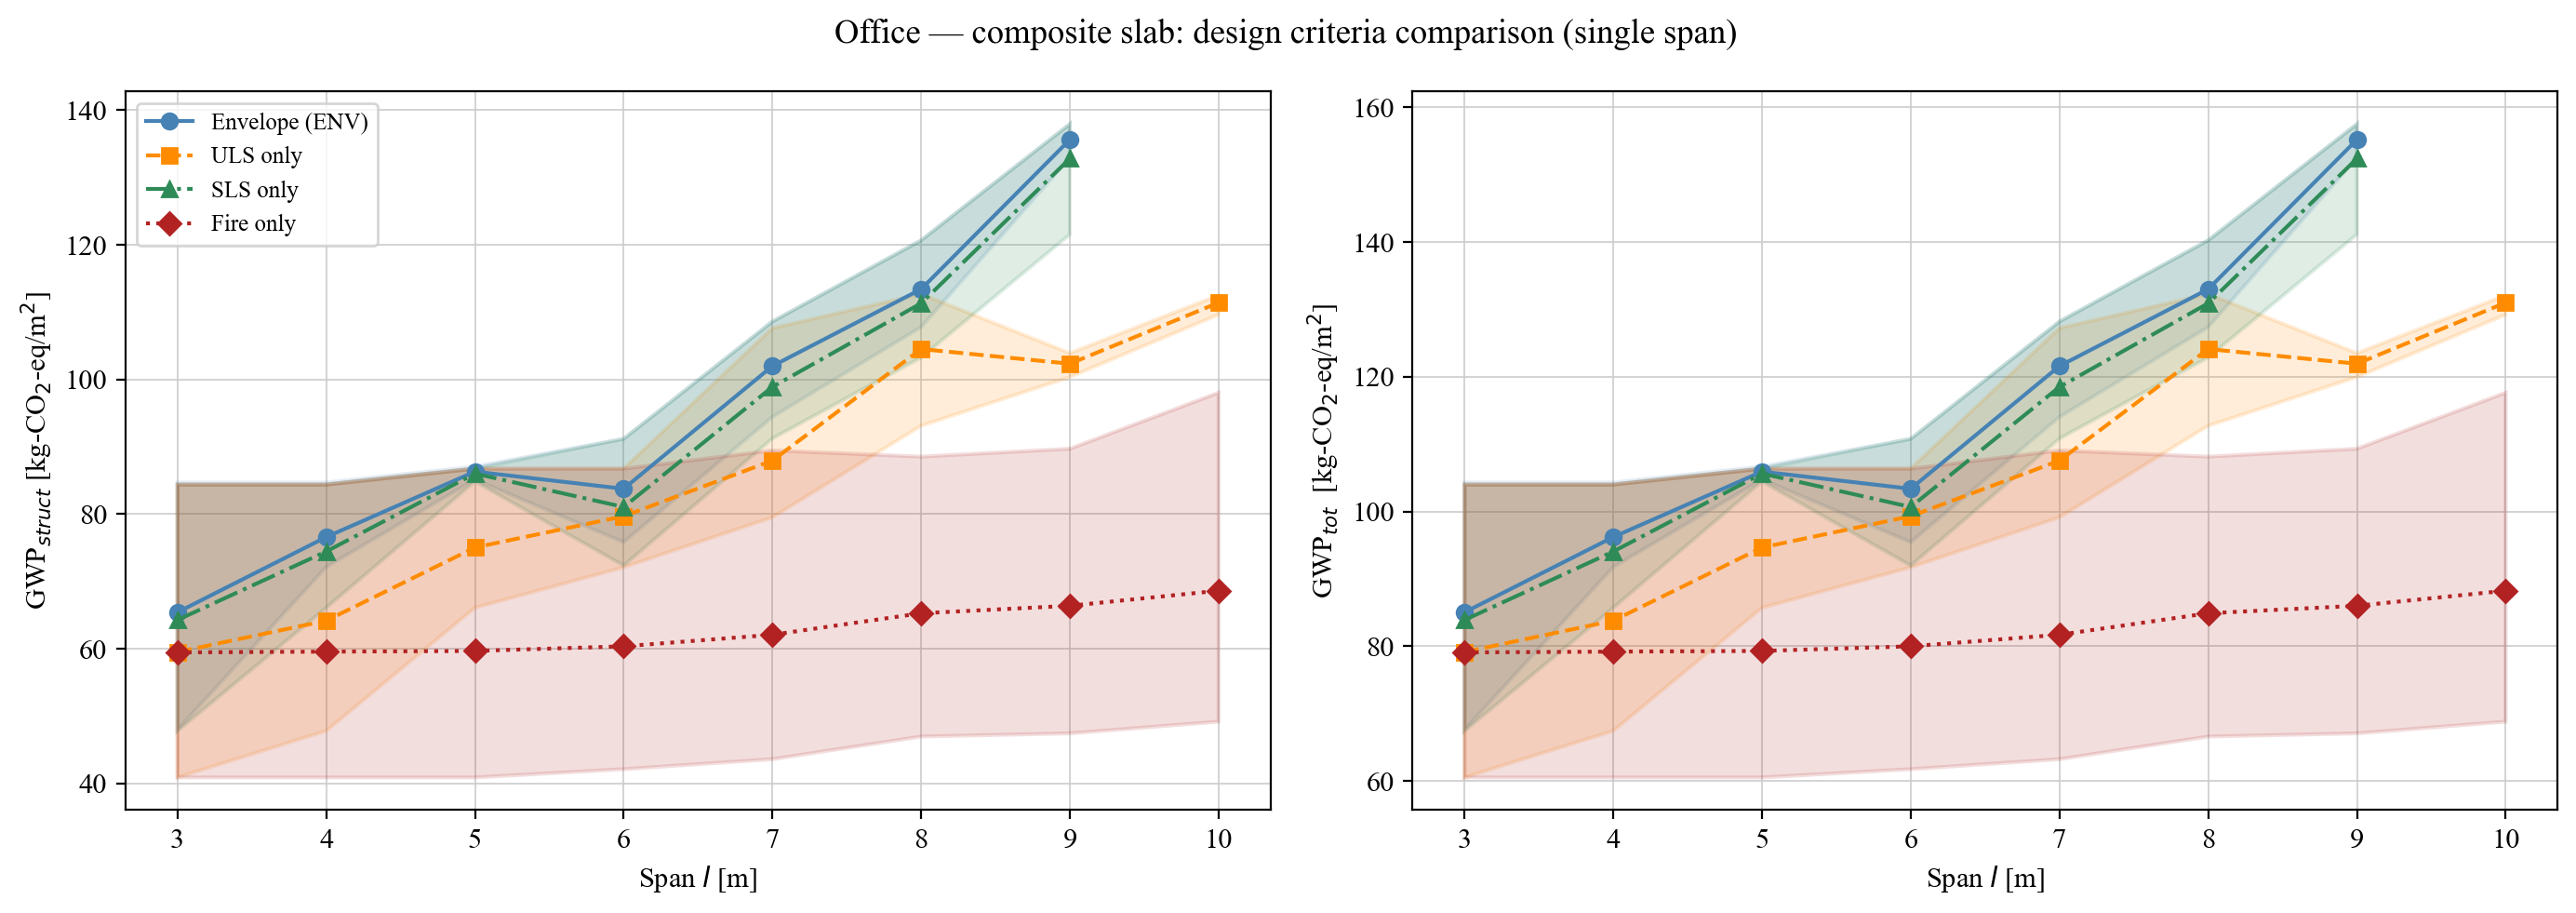
\includegraphics[width=\textwidth]{figures/office/fig_criteria_comparison_SS.png}
        \caption{Single span}
        \label{fig:office_criteria_SS}
    \end{subfigure}\\[4pt]
    \begin{subfigure}{\textwidth}
        \centering
        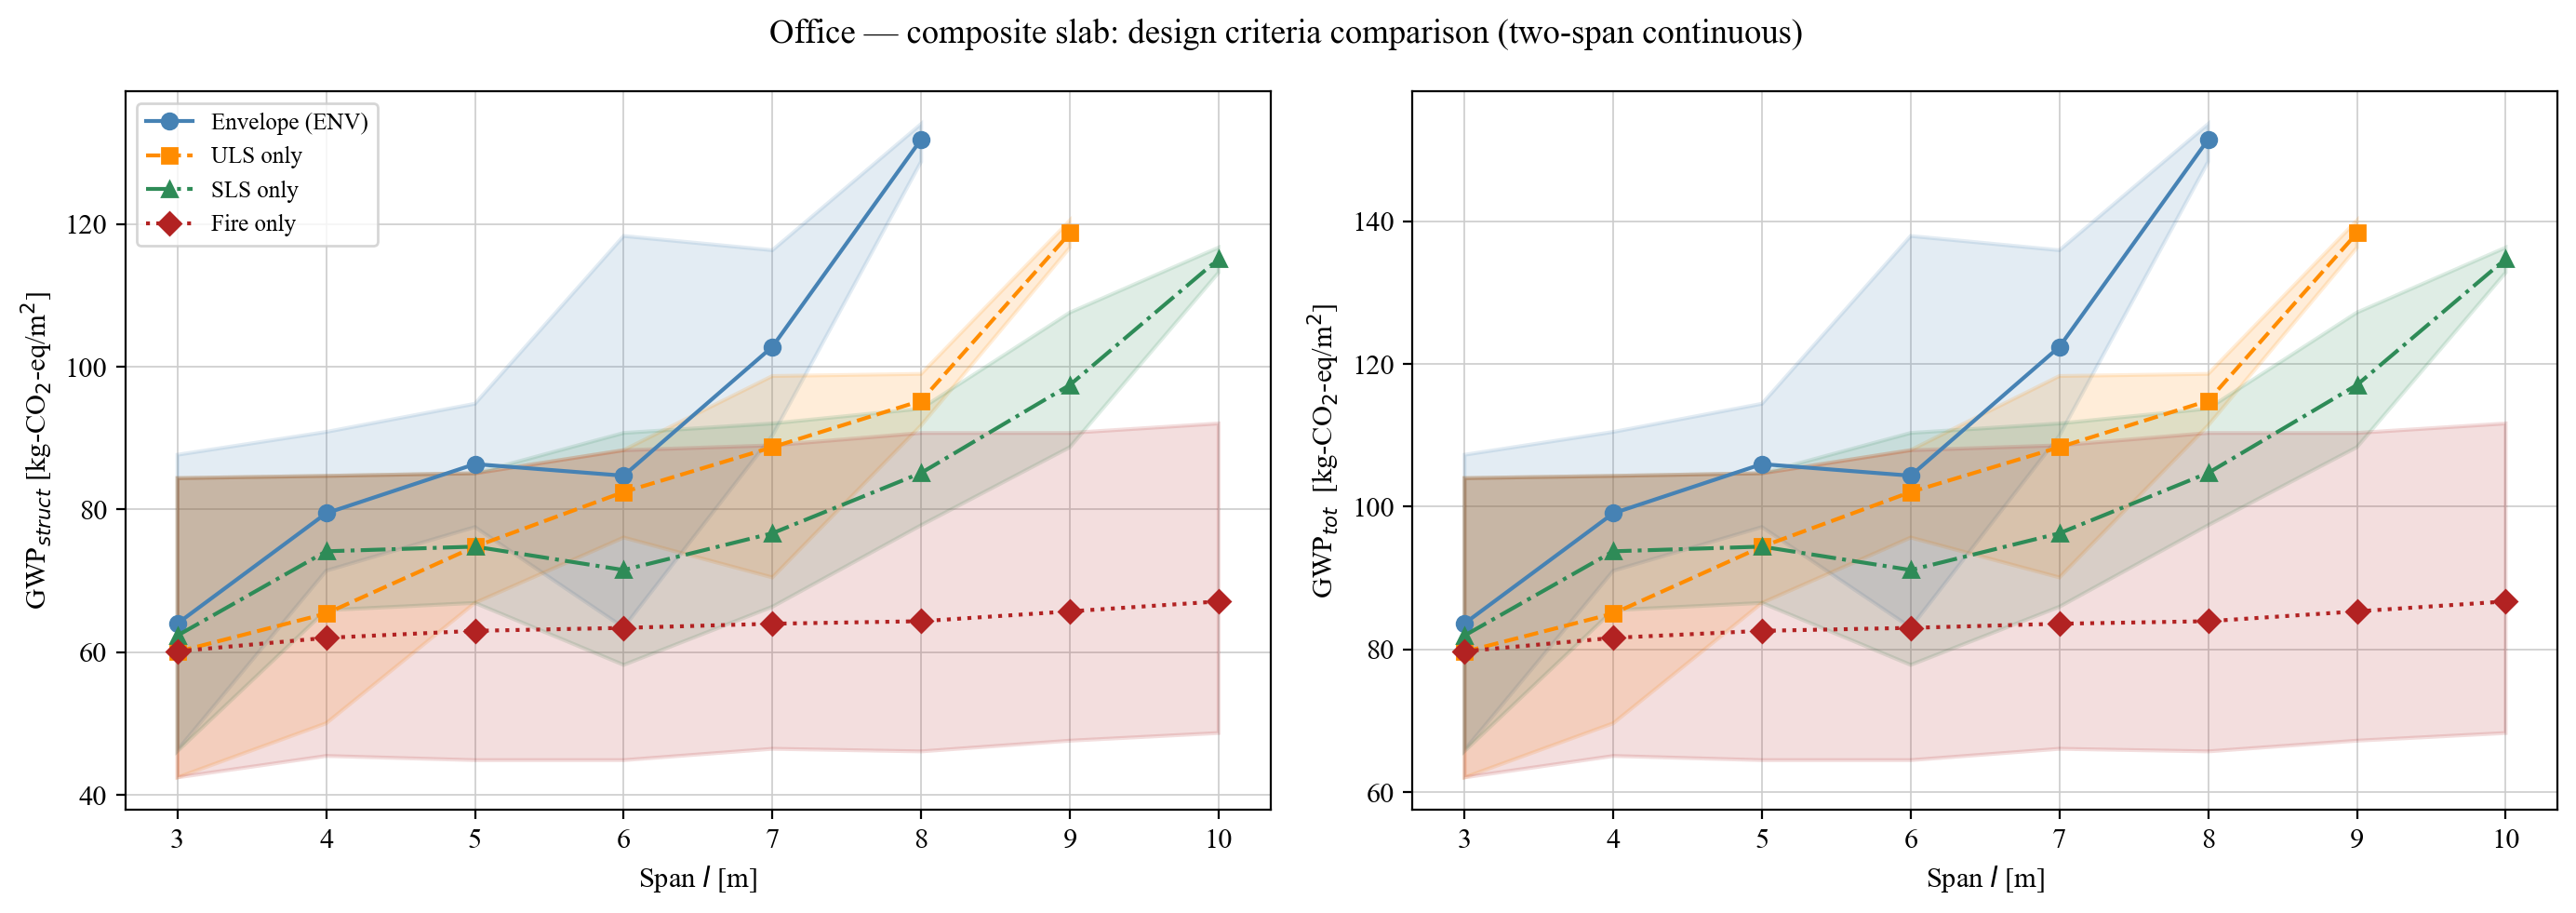
\includegraphics[width=\textwidth]{figures/office/fig_criteria_comparison_2span.png}
        \caption{Two--span continuous}
        \label{fig:office_criteria_2span}
    \end{subfigure}\\[4pt]
    \begin{subfigure}{\textwidth}
        \centering
        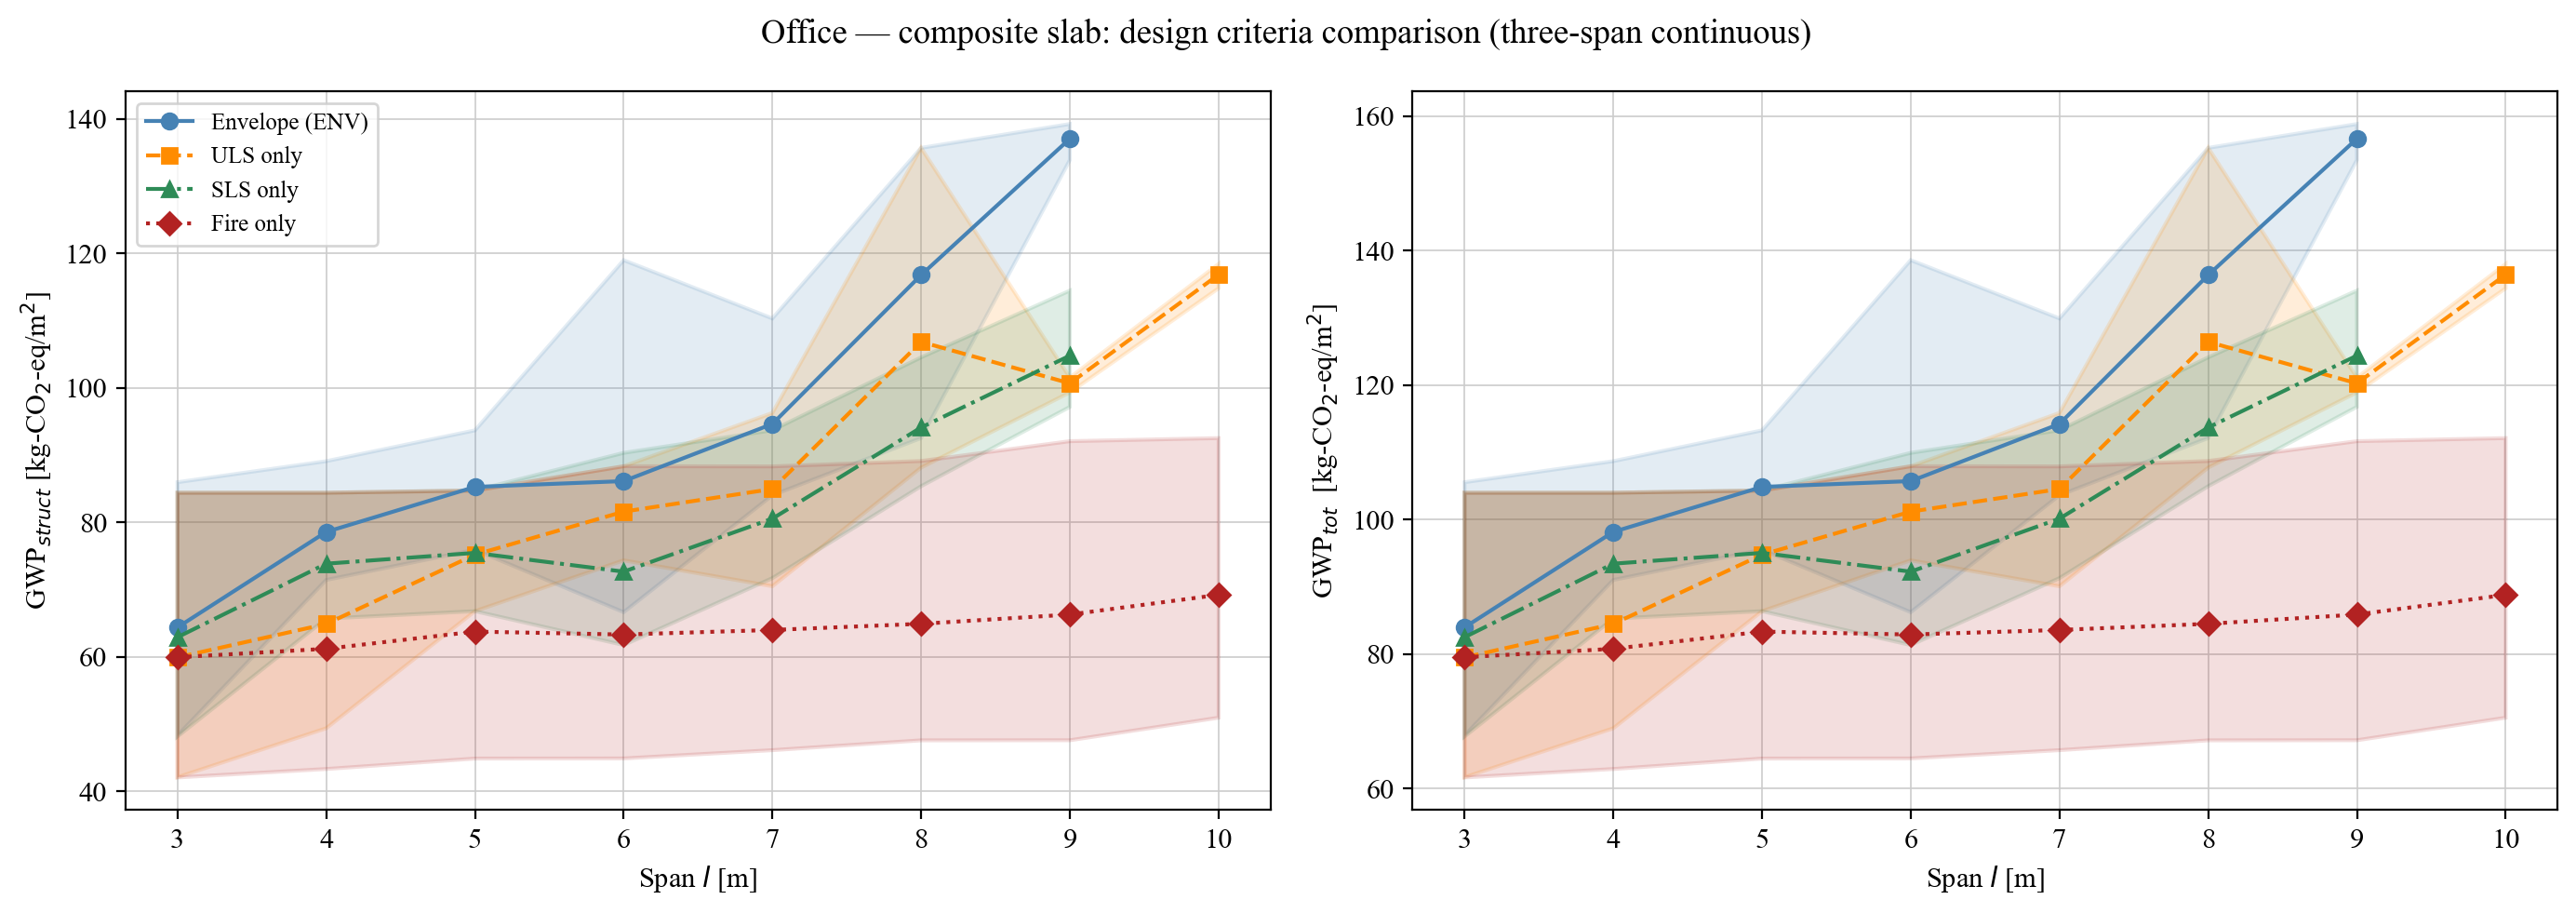
\includegraphics[width=\textwidth]{figures/office/fig_criteria_comparison_3span.png}
        \caption{Three--span continuous}
        \label{fig:office_criteria_3span}
    \end{subfigure}
    \caption[Office composite design criteria comparison]{Office composite slab: GWP of the optima obtained under each design criterion in isolation (ULS only, SLS only, fire only) compared with the combined envelope (ENV), for the single--, two--, and three--span configurations.}
    \label{fig:office_criteria}
\end{figure}

Examining the feasible solution space shows that unpropped construction is feasible only up to 5\,m in every span configuration. At 3\,m, 32 deck--grade combinations satisfy all checks unpropped (single span); this falls to 16 at 4\,m and just 4 at 5\,m, and from 6\,m upward no deck in the database can carry the wet--concrete construction load unpropped within the 300\,mm depth bound. The two-- and three--span configurations show the same cliff at 6\,m, with marginally more unpropped options surviving at 5\,m (8 each) because continuity of the bare deck over the supports slightly reduces the construction--stage sagging moment. Since the construction stage is carried by the steel deck alone---before composite action develops---the number of final spans has little influence on where unpropped construction runs out.

Critically, propping lowers GWP even at spans where unpropped construction remains feasible. At 3\,m the lightest feasible unpropped single--span section carries 67.6\,kg\,CO$_2$eq/m$^2$ against 61.8 propped; at 5\,m the gap widens to 104.7 versus 83.8\,kg\,CO$_2$eq/m$^2$. Unpropped construction forces a heavier, deeper deck purely to survive the wet--concrete pour, whereas propping removes that constraint and allows the section to be sized by the in--service limit states. Propping therefore would be selected throughout the office range below 6\,m because it yields the lower--carbon section, if the unpropped preference encoded in the optimisation routine were not applied.

The upper feasibility limit differs by configuration. The single-- and three--span cases remain feasible (propped) up to 9\,m, but the \textbf{two--span configuration becomes infeasible beyond 8\,m}---one span sooner---because the hogging moment at the single internal support is the most severe of the three arrangements, and no deck--reinforcement combination can satisfy the hogging ULS and fire D3 checks at 9\,m within the depth bound. The three--span case distributes the support moments more favourably and recovers feasibility at 9\,m. No configuration is feasible at 10\,m: at that span the composite SLS deflection check cannot be satisfied within the 500\,mm depth bound for any deck in the database, even with propped construction.

%------------------------------------------------------------------
\subsubsection{GWP breakdown by material}
\label{sec:res_office_breakdown}
%------------------------------------------------------------------
Table~\ref{tab:office_breakdown} decomposes the single--span composite GWP into its material contributions. The steel deck is the single largest structural contributor at most spans, exceeding the concrete contribution up to 6\,m and remaining comparable beyond it, despite the steel mass being far smaller than the concrete mass---a direct consequence of the much higher GWP intensity per kilogram of structural steel. The fixed floor build--up (19.6\,kg\,CO$_2$eq/m$^2$) is 32\% of the total at 3\,m but only 13\% at 9\,m, as the structural contribution grows with span.

\begin{table}[h!]
\small\centering
\caption{GWP breakdown of the optimal composite slab, office single span (kg\,CO$_2$eq/m$^2$).}
\label{tab:office_breakdown}
\begin{tabular}{ccccccc}
\toprule
$L$ [m] & Concrete & Deck & Mesh & Trough bars & Struct. & Build--up \\
\midrule
3 & 15.1 & 23.4 & 1.6 & 2.2  & 42.2  & 19.6 \\
4 & 19.2 & 28.8 & 2.4 & 2.4  & 52.7  & 19.6 \\
5 & 28.9 & 29.2 & 2.4 & 3.7  & 64.2  & 19.6 \\
6 & 24.8 & 46.9 & 2.4 & 1.7  & 75.8  & 19.6 \\
7 & 41.2 & 49.1 & 2.4 & 1.7  & 94.4  & 19.6 \\
8 & 53.2 & 49.1 & 2.4 & 3.1  & 107.8 & 19.6 \\
9 & 54.9 & 60.8 & 2.4 & 14.8 & 132.9 & 19.6 \\
\bottomrule
\end{tabular}
\end{table}

The fire trough--bar contribution is small at most spans but jumps to 14.8\,kg\,CO$_2$eq/m$^2$ at 9\,m, where the deep section requires substantial trough reinforcement to satisfy the D2 fire sagging check. Figure~\ref{fig:office_breakdown} shows the breakdown as a stacked bar for the single span; the equivalent figures for the two-- and three--span configurations are given in Appendix~\ref{app:results_figures}.

\begin{figure}[h!]
    \centering
    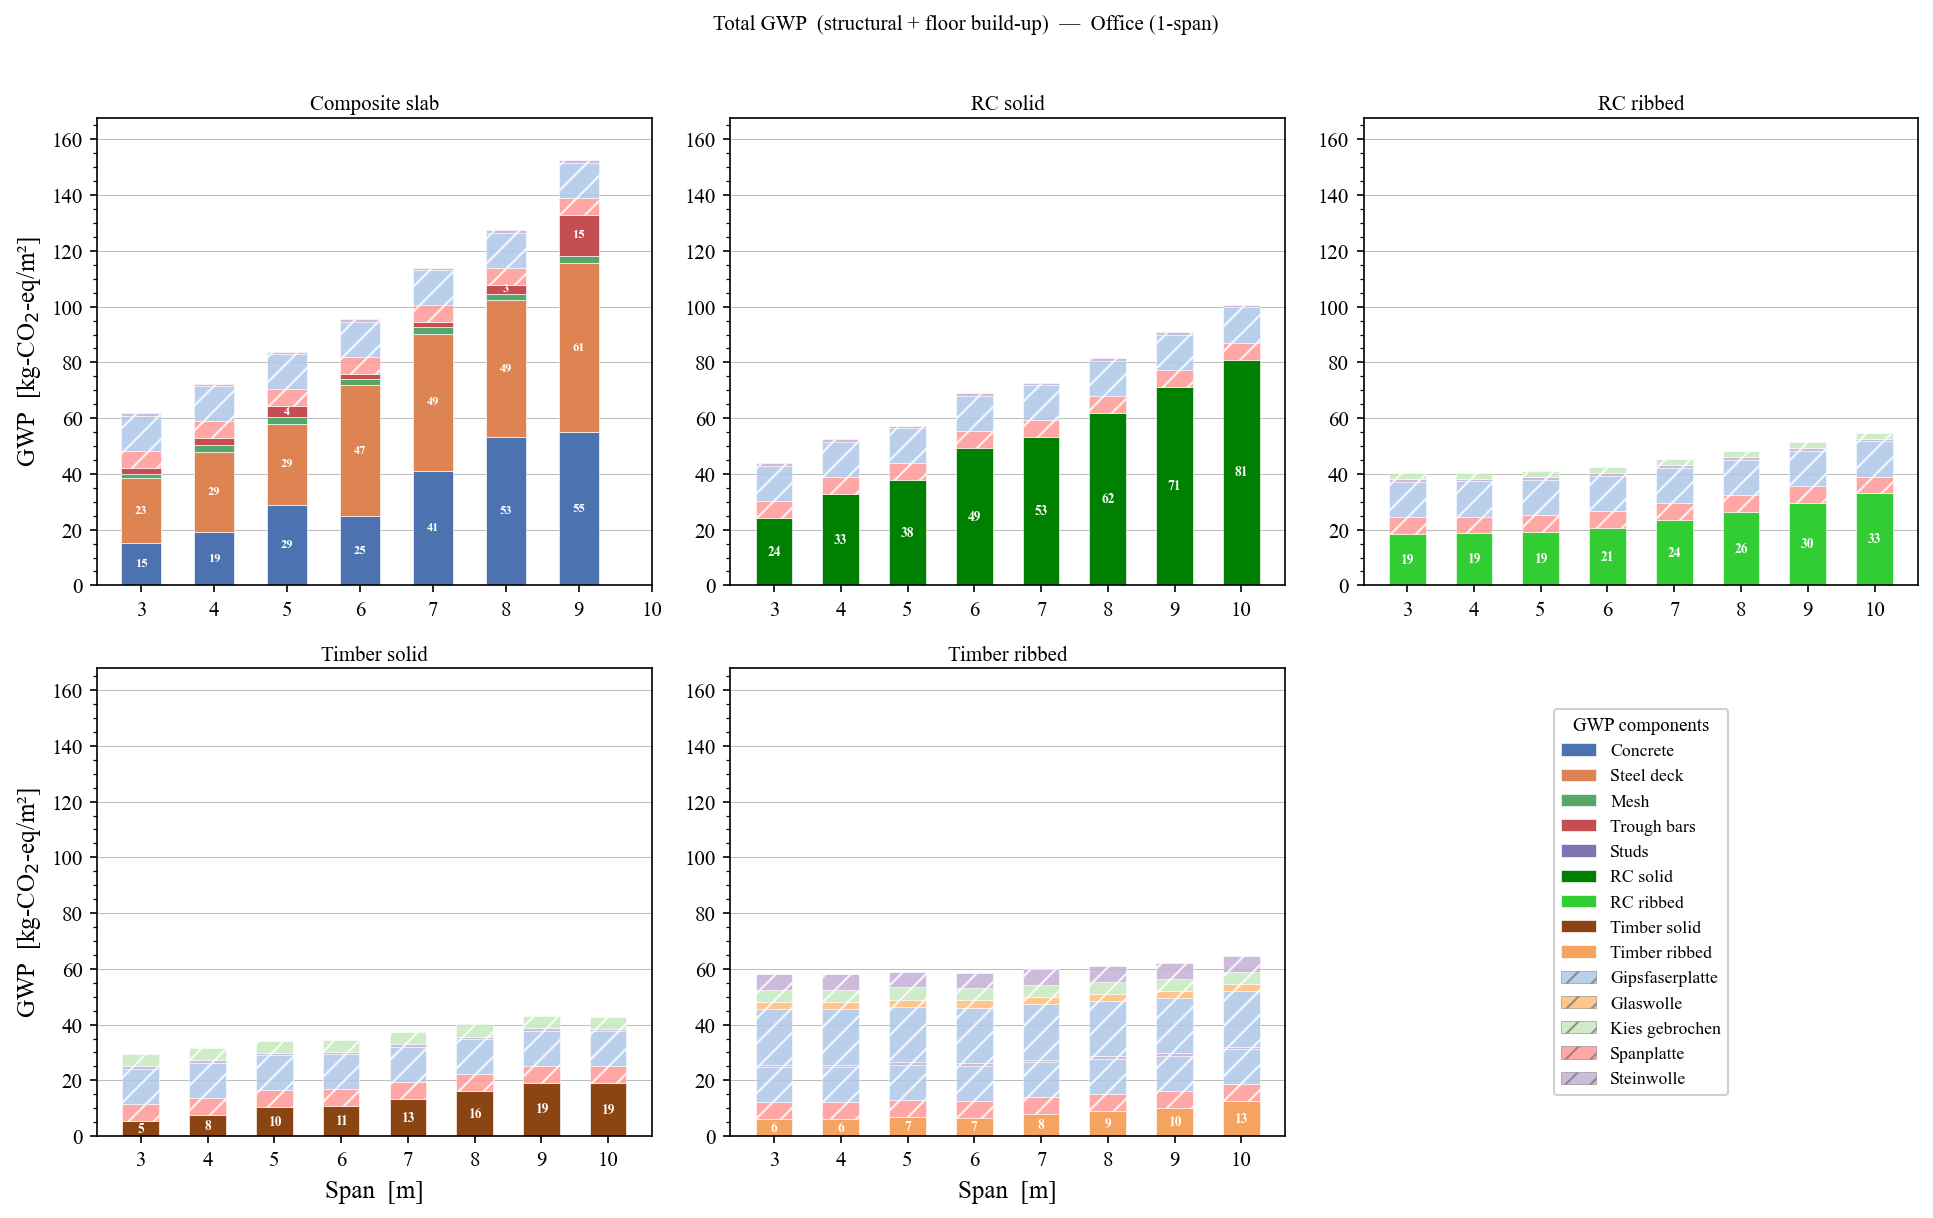
\includegraphics[width=\textwidth]{figures/office/GWP breakdown/results_office_ENV_gwp_total.png}
    \caption[Office GWP breakdown, single span]{Office single span: total GWP of the optimal slab.}
    \label{fig:office_breakdown}
\end{figure}

%------------------------------------------------------------------
\subsubsection{Structural depth and mass}
\label{sec:res_office_depth}
%------------------------------------------------------------------
Figure~\ref{fig:office_height} compares the structural depth ($h_\mathrm{struct}$) and total depth ($h_\mathrm{tot}$, including the floor build--up) of the five systems against span, for all three span configurations. The composite curve distinguishes the unpropped optimum (feasible only to 5\,m) from the propped optimum, which is the governing optimum across the full range (Section~\ref{sec:res_office_gov}).

\begin{figure}[h!]
    \centering
    \begin{subfigure}{\textwidth}
        \centering
        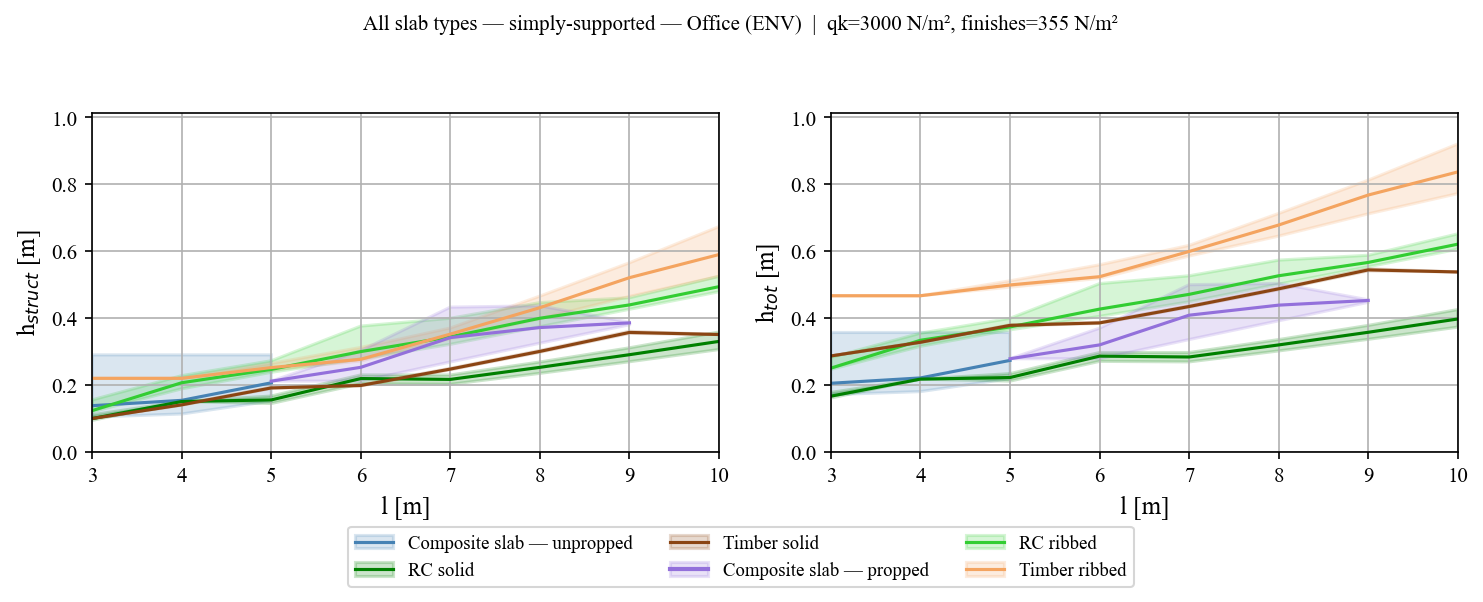
\includegraphics[width=\textwidth]{figures/office/ENV/plot_office_1span_ENV_height.png}
        \caption{Single span}
        \label{fig:office_height_SS}
    \end{subfigure}\\[4pt]
    \begin{subfigure}{\textwidth}
        \centering
        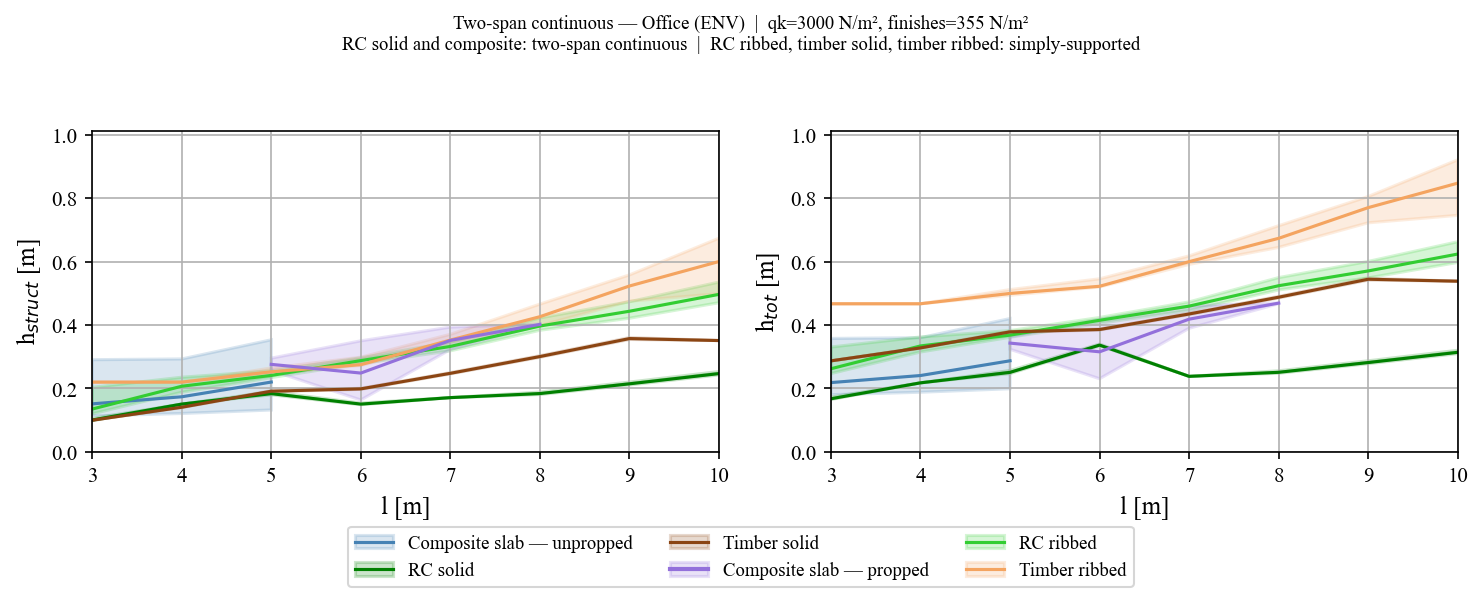
\includegraphics[width=\textwidth]{figures/office/ENV/plot_office_2span_ENV_height.png}
        \caption{Two--span continuous}
        \label{fig:office_height_2span}
    \end{subfigure}\\[4pt]
    \begin{subfigure}{\textwidth}
        \centering
        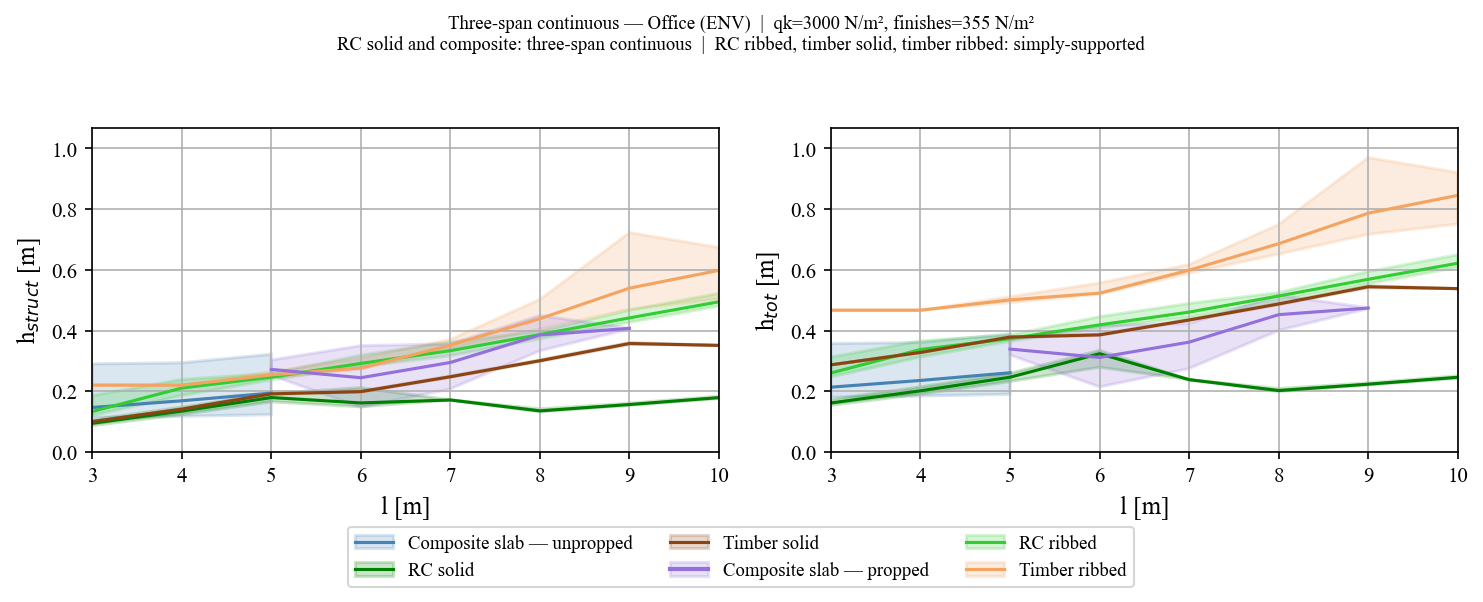
\includegraphics[width=\textwidth]{figures/office/ENV/plot_office_3span_ENV_height.png}
        \caption{Three--span continuous}
        \label{fig:office_height_3span}
    \end{subfigure}
    \caption[Office slab depth versus span]{Office scenario: structural depth $h_\mathrm{struct}$ (left) and total depth $h_\mathrm{tot}$ (right) versus span for all five systems, in the single--, two--, and three--span configurations.}
    \label{fig:office_height}
\end{figure}

The optimal composite depth grows with span in two distinct regimes. At short spans the section is shallow and nearly constant across configurations---the single--, two--, and three--span optima are all 180--185\,mm total at 3\,m---because the depth here is set by the fire thermal--insulation minimum rather than by strength or stiffness. As span increases, the optimiser selects a shallow trapezoidal deck (ComFlor~60, Multideck~80) until the deflection limit (single span) or the support hogging check (continuous spans) can no longer be met, at which point it steps abruptly to a deep deck (ComFlor~210/225). This produces a characteristic jump in depth: for the single span the total depth rises from 249\,mm at 5\,m to 365\,mm at 6\,m, whereas the continuous configurations select a shallow section for one span further---233--240\,mm at 6\,m---before jumping to roughly 400--430\,mm at 7\,m. Continuity therefore defers the transition to deep decking by approximately one span, because the reduced sagging moment over continuous supports keeps the shallow deck viable for longer.

Relative to the other systems, the composite slab is competitive on total depth despite its high embodied carbon. At the longest feasible spans its total depth (around 455\,mm at 9\,m, single span) is the second--shallowest of the five systems, exceeded only by the RC flat slab and sitting well below the RC ribbed and both timber systems. This shallow structural depth is one of the practical advantages of composite construction that the carbon comparison alone does not capture, and is returned to in the discussion (Chapter~\ref{fifthchapter}).

Grade C25/30 is selected in every optimum except the 6\,m three--span case, confirming that the section is not concrete--strength--governed; a stronger grade offers negligible structural benefit at higher GWP intensity.

The structural mass of the optimal sections is shown in Figure~\ref{fig:office_mass}. Broadly the mass tracks GWP, as expected since embodied carbon scales with material quantity, but the correspondence is not exact and the divergences are informative.
 
\begin{figure}[h!]
    \centering
    \begin{subfigure}{\textwidth}
        \centering
        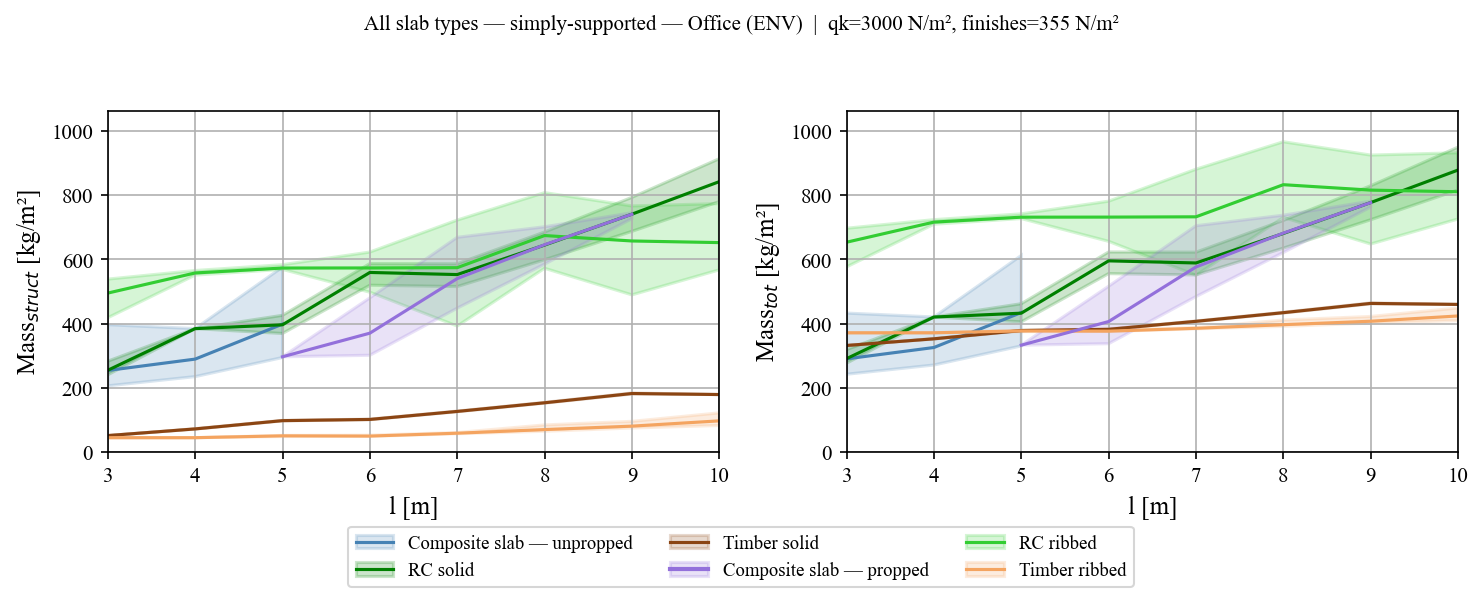
\includegraphics[width=\textwidth]{figures/office/ENV/plot_office_1span_ENV_mass.png}
        \caption{Single span}
        \label{fig:office_mass_SS}
    \end{subfigure}\\[4pt]
    \begin{subfigure}{\textwidth}
        \centering
        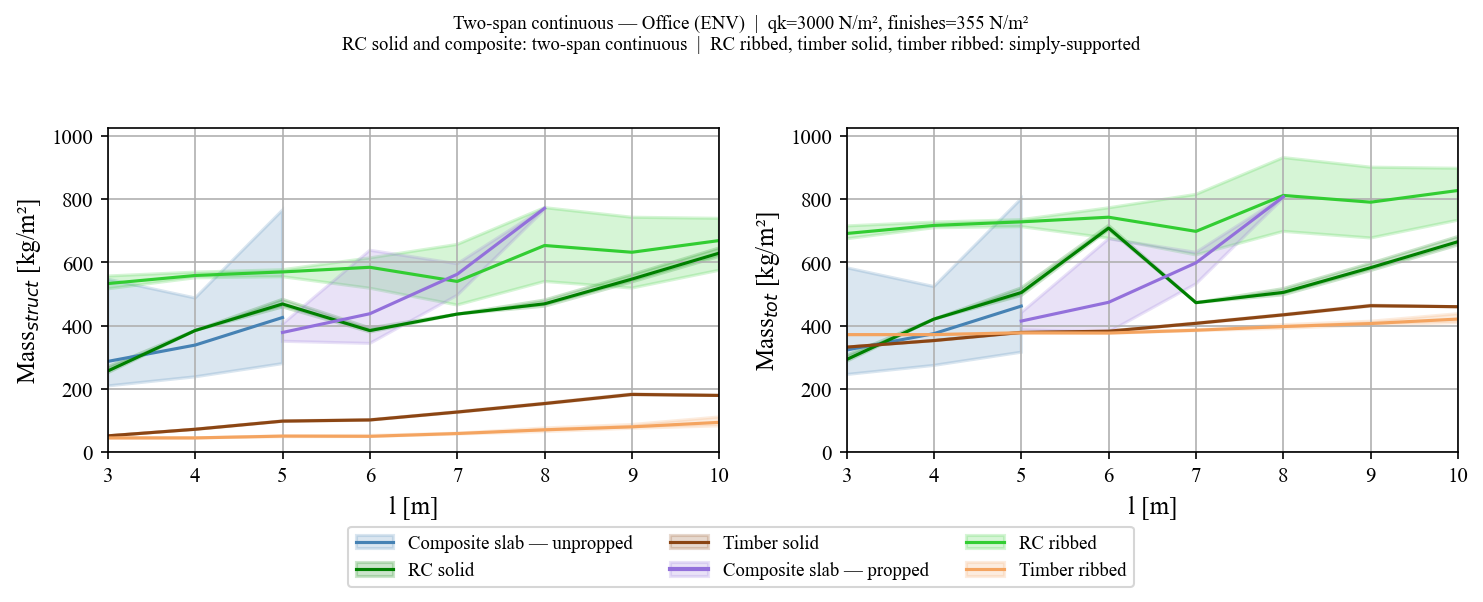
\includegraphics[width=\textwidth]{figures/office/ENV/plot_office_2span_ENV_mass.png}
        \caption{Two--span continuous}
        \label{fig:office_mass_2span}
    \end{subfigure}\\[4pt]
    \begin{subfigure}{\textwidth}
        \centering
        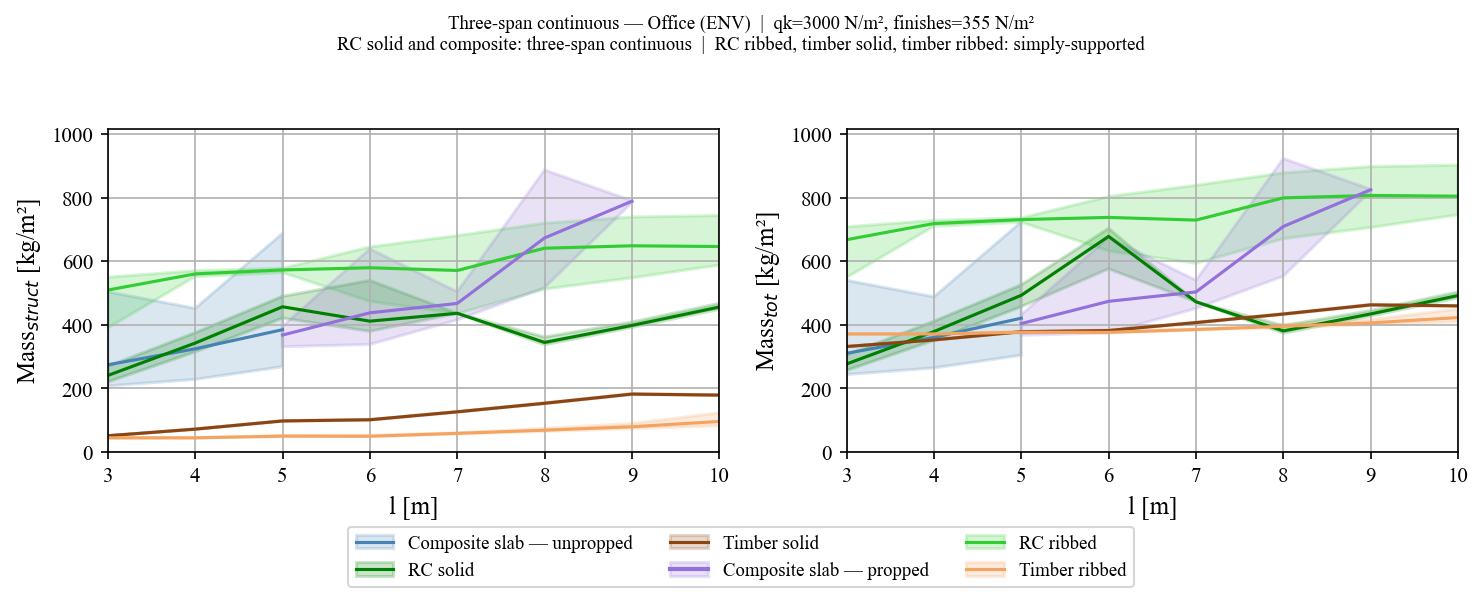
\includegraphics[width=\textwidth]{figures/office/ENV/plot_office_3span_ENV_mass.png}
        \caption{Three--span continuous}
        \label{fig:office_mass_3span}
    \end{subfigure}
    \caption[Office slab mass versus span]{Office scenario: structural mass $\mathrm{Mass}_\mathrm{struct}$ (left) and total mass $\mathrm{Mass}_\mathrm{tot}$ (right) per unit floor area versus span for all five systems, in the single--, two--, and three--span configurations.}
    \label{fig:office_mass}
\end{figure}
 
The composite slab is a heavy floor system, comparable in mass to reinforced concrete and far heavier than timber. The single--span composite optimum rises from 242\,kg/m$^2$ at 3\,m to 781\,kg/m$^2$ at 9\,m, almost entirely concrete; over the same range the two timber systems remain between roughly 370 and 460\,kg/m$^2$, so the composite slab is approximately twice the mass of an equivalent timber floor at the longer spans. This is a direct consequence of the cast in--situ concrete, which dominates the cross--section by mass even though the steel deck dominates by embodied carbon.
 
The most important observation is that mass and GWP do not rank the systems identically. The composite slab carries \textit{less} structural mass than the RC flat slab at the longer spans---745\,kg/m$^2$ against roughly 840\,kg/m$^2$ at 9\,m---yet has a substantially higher GWP. The composite slab's carbon penalty therefore arises from the high embodied--carbon intensity of the profiled steel deck per kilogram, not from the quantity of material in the floor. This reinforces the GWP breakdown of Section~\ref{sec:res_office_breakdown}, in which the steel deck is the largest single contributor to structural GWP despite being a small fraction of the mass.
 
This mass has consequences beyond embodied carbon---for foundation and column loads, and for the seismic mass of the structure---that are considered in the discussion (Chapter~\ref{fifthchapter}).

%------------------------------------------------------------------
\subsubsection{Effect of span continuity}
\label{sec:res_office_continuity}
%------------------------------------------------------------------
Figure~\ref{fig:office_continuity} plots the composite GWP optimum for the single--, two--, and three--span configurations on a single axis. The effect of continuity on the composite slab is small and non--monotonic, and it contrasts sharply with the reinforced concrete flat slab, for which continuity reduces GWP increasingly with span.

\begin{figure}[h!]
    \centering
    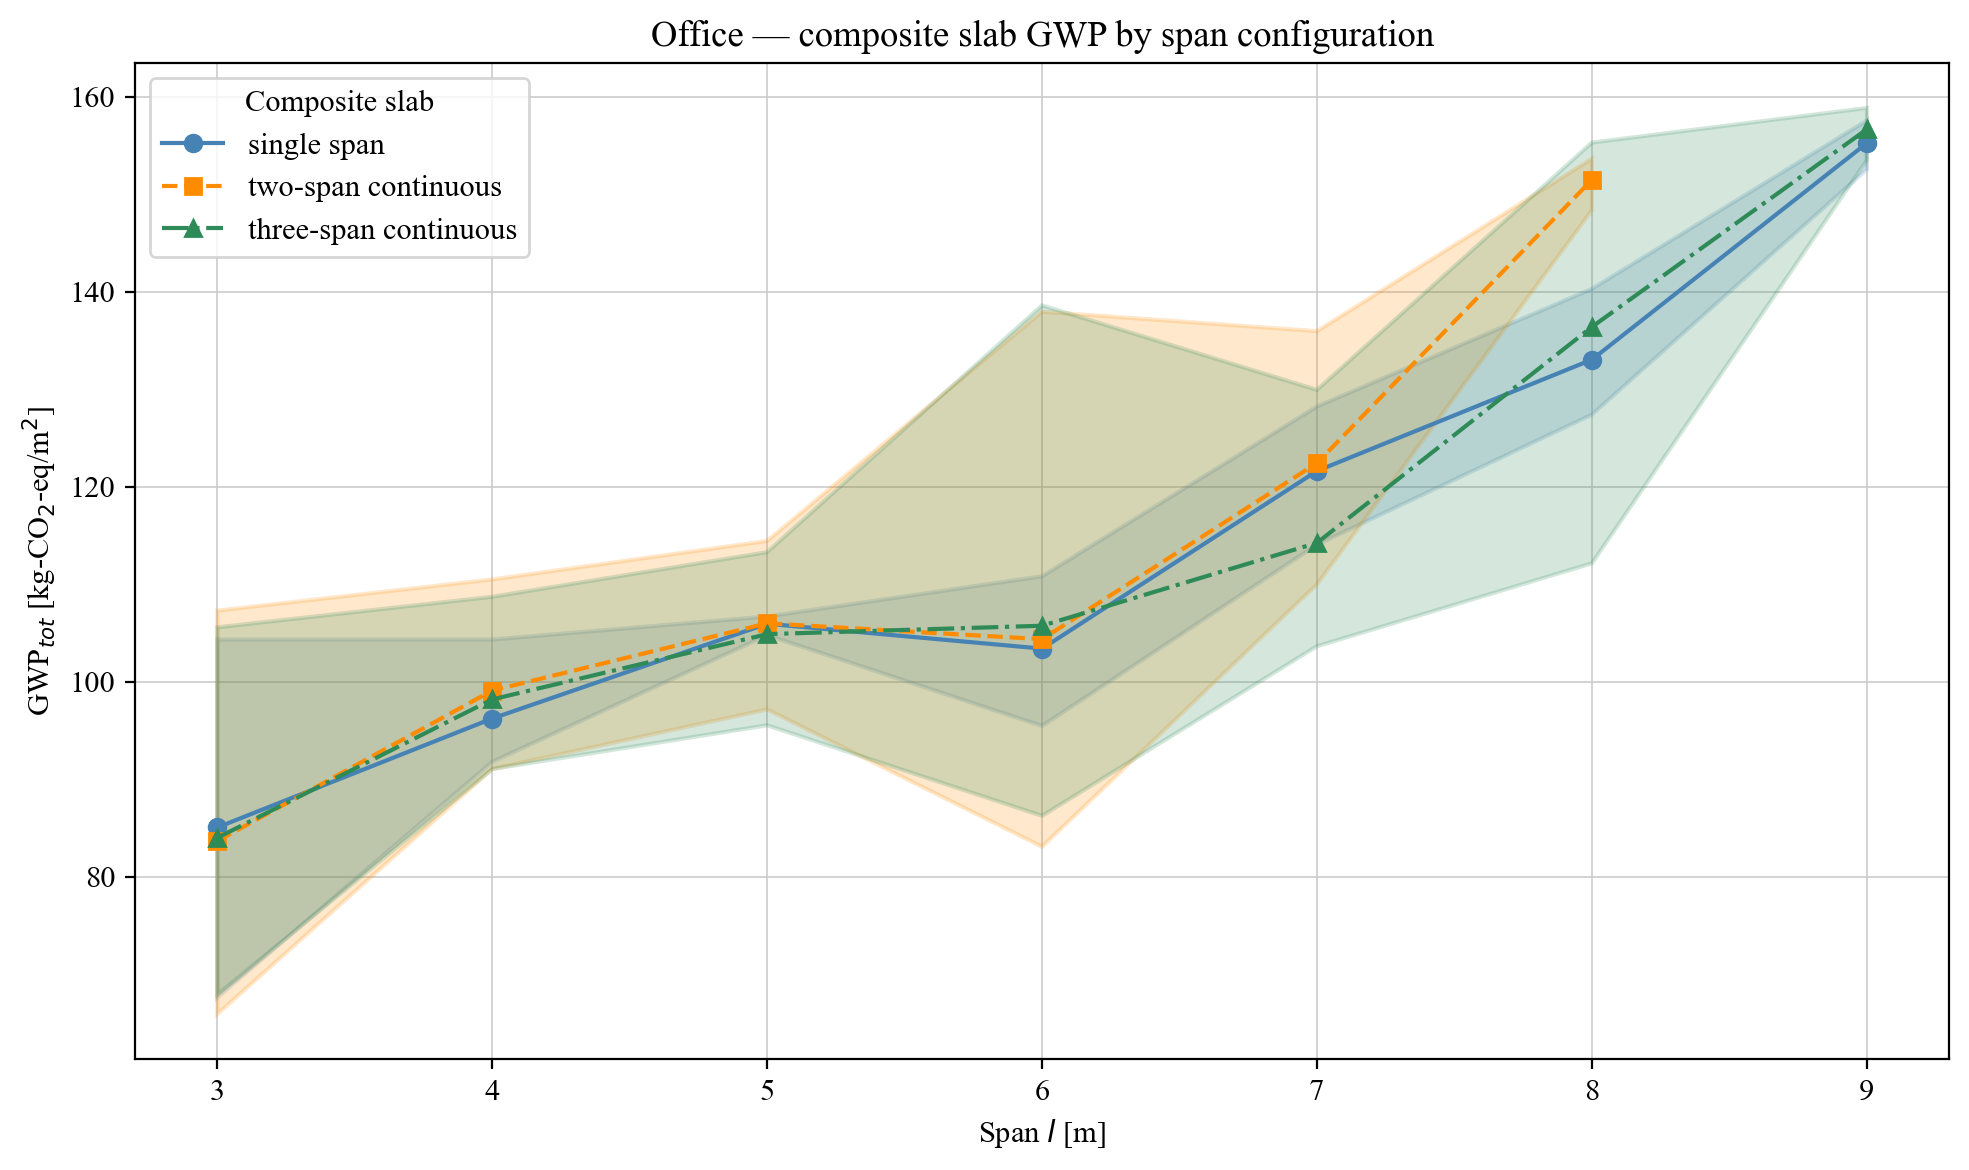
\includegraphics[width=0.85\textwidth]{figures/fig_composite_span_configs.png}
    \caption[Office composite GWP by span configuration]{Office composite slab: total GWP versus span for the single--, two--, and three--span configurations. Shaded bands show the spread of feasible solutions at each span; markers are the GWP optima.}
    \label{fig:office_continuity}
\end{figure}

Up to 6\,m the three configurations are almost indistinguishable: the optima differ by at most a few kg\,CO$_2$eq/m$^2$, and their feasibility envelopes overlap almost completely. The configuration effect emerges only at the longer spans: at 8\,m the three--span optimum (112.1) is the lowest, the single span (127.4) is intermediate, and the two--span case is the highest at 148.4\,kg\,CO$_2$eq/m$^2$ ---higher than the single span, despite being continuous. The two--span configuration also becomes infeasible beyond 8\,m, whereas the single-- and three--span cases reach 9\,m and converge there at around 152--154\,kg\,CO$_2$eq/m$^2$.

%==============================================================================
\subsection{Other occupancy scenarios}
\label{sec:res_other}
%==============================================================================
The residential, retail, and industrial scenarios reproduce the office findings: the composite slab is the highest--carbon system at every span, the ranking of the five systems is unchanged, and the composite design is stiffness-- or hogging--governed over most of the range. Only the differences from the office case are reported here; full figures and tables are in Appendix~\ref{app:results_figures}.

\subsubsection{Residential}
\label{sec:res_residential}
The residential scenario carries a higher imposed load ($q_k = 2.0$\,kN/m$^2$) and a heavier screed-based build-up (+26.4\,kg\,CO$_2$eq/m$^2$), raising all systems' GWP relative to office. The optimal composite cross-sections are listed in Table~\ref{tab:residential_optima}. The single-span composite optimum runs from 80.2 at 3\,m to 165.8\,kg\,CO$_2$eq/m$^2$ at 9\,m; no feasible solution exists at 10\,m. The ranking across the five systems and the governing limit states are unchanged from the office case. Fire D1 governs at 3\,m, fire checks (D2--D4) govern at 4--5\,m, and SLS deflection or hogging governs from 6\,m upward. The composite-to-RC-ribbed gap is again roughly 45\% at short spans, widening with span.

\begin{table}[h!]
\small\centering
\caption{Optimal composite cross--sections, residential scenario, all span configurations.}
\label{tab:residential_optima}
\begin{tabular}{llcccccl}
\toprule
Config. & $L$ [m] & Deck & Grade & $h$ [mm] & $\mathrm{GWP}_\mathrm{tot}$ & Propped & Governing check \\
\midrule
\multirow{7}{*}{Single}
 & 3 & Multideck 80 1.1  & C25/30 & 131 & 80.2  & No  & Fire D1 \\
 & 4 & ComFlor 210       & C25/30 & 290 & 101.5 & No  & Fire D4 \\
 & 5 & ComFlor 60 0.9    & C25/30 & 200 & 97.0  & Yes & Fire D2 \\
 & 6 & ComFlor 210       & C25/30 & 319 & 109.2 & Yes & SLS deflection \\
 & 7 & ComFlor 225       & C25/30 & 392 & 128.5 & Yes & SLS deflection \\
 & 8 & ComFlor 225       & C25/30 & 463 & 142.0 & Yes & ULS long.\ shear \\
 & 9 & Multideck 146 1.5 & C25/30 & 406 & 165.8 & Yes & SLS deflection \\
\midrule
\multirow{6}{*}{Two--span}
 & 3 & Multideck 80 1.0  & C25/30 & 140 & 79.7  & No  & Fire D3 \\
 & 4 & ComFlor 210       & C25/30 & 307 & 104.3 & No  & Fire D2 \\
 & 5 & ComFlor 225       & C25/30 & 313 & 110.3 & No  & Fire D3 \\
 & 6 & ComFlor 60 1.0    & C25/30 & 184 & 101.4 & Yes & ULS hogging \\
 & 7 & ComFlor 210       & C25/30 & 392 & 125.1 & Yes & Fire D3 \\
 & 8 & Multideck 146 1.5 & C25/30 & 448 & 166.7 & Yes & ULS hogging \\
\midrule
\multirow{6}{*}{Three--span}
 & 3 & Multideck 80 1.0  & C25/30 & 140 & 79.4  & No  & Fire D3 \\
 & 4 & ComFlor 210       & C25/30 & 297 & 102.8 & No  & Fire D3 \\
 & 5 & ComFlor 225       & C25/30 & 302 & 108.0 & No  & Fire D3 \\
 & 6 & ComFlor 60 1.0    & C25/30 & 185 & 101.7 & Yes & ULS hogging \\
 & 7 & ComFlor 210       & C25/30 & 351 & 117.7 & Yes & Fire D3 \\
 & 8 & ComFlor 210       & C25/30 & 403 & 128.9 & Yes & Fire D3 \\
\bottomrule
\end{tabular}
\end{table}

\subsubsection{Retail}
\label{sec:res_retail}
The retail scenario uses the same elevated imposed load ($q_k = 4.0$\,kN/m$^2$) as residential but a lighter parquet-and-board build-up (+19.0\,kg\,CO$_2$eq/m$^2$). The optimal cross-sections are listed in Table~\ref{tab:retail_optima}. The single-span composite optimum runs from 70.6 at 3\,m to 156.3\,kg\,CO$_2$eq/m$^2$ at 9\,m. Governing limit states follow the office and residential pattern: fire governs at short spans, SLS deflection or hogging from 6\,m upward. The two-span configuration becomes infeasible beyond 7\,m (one span earlier than the office case), because the higher imposed load increases the hogging demand at the single internal support. The three-span configuration remains feasible to 8\,m.

\begin{table}[h!]
\small\centering
\caption{Optimal composite cross--sections, retail scenario, all span configurations.}
\label{tab:retail_optima}
\begin{tabular}{llcccccl}
\toprule
Config. & $L$ [m] & Deck & Grade & $h$ [mm] & $\mathrm{GWP}_\mathrm{tot}$ & Propped & Governing check \\
\midrule
\multirow{7}{*}{Single}
 & 3 & Multideck 80 1.0  & C25/30 & 131 & 70.6  & No  & Fire D1 \\
 & 4 & ComFlor 210       & C25/30 & 290 & 94.7  & No  & Fire D4 \\
 & 5 & Multideck 146 1.5 & C25/30 & 212 & 107.7 & No  & Fire D4 \\
 & 6 & ComFlor 210       & C25/30 & 309 & 100.5 & Yes & SLS deflection \\
 & 7 & ComFlor 225       & C25/30 & 380 & 119.5 & Yes & SLS deflection \\
 & 8 & Multideck 146 1.2 & C25/30 & 408 & 147.1 & Yes & ULS long.\ shear \\
 & 9 & Multideck 146 1.5 & C25/30 & 392 & 156.3 & Yes & SLS deflection \\
\midrule
\multirow{5}{*}{Two--span}
 & 3 & Multideck 80 1.0  & C25/30 & 139 & 80.4  & No  & Fire D3 \\
 & 4 & ComFlor 210       & C25/30 & 321 & 107.7 & No  & Fire D3 \\
 & 5 & ComFlor 60 0.9    & C25/30 & 166 & 92.9  & Yes & ULS hogging \\
 & 6 & ComFlor 60 1.0    & C30/37 & 206 & 107.9 & Yes & ULS hogging \\
 & 7 & ComFlor 210       & C25/30 & 431 & 133.0 & Yes & ULS hogging \\
\midrule
\multirow{6}{*}{Three--span}
 & 3 & Multideck 80 1.0  & C25/30 & 133 & 79.2  & No  & Fire D3 \\
 & 4 & ComFlor 210       & C25/30 & 307 & 105.0 & No  & Fire D3 \\
 & 5 & ComFlor 60 0.9    & C25/30 & 159 & 91.6  & Yes & ULS hogging \\
 & 6 & ComFlor 80 0.9    & C25/30 & 205 & 104.3 & Yes & ULS hogging \\
 & 7 & ComFlor 210       & C25/30 & 378 & 123.0 & Yes & Fire D3 \\
 & 8 & Multideck 146 1.5 & C25/30 & 407 & 163.0 & Yes & ULS hogging \\
\bottomrule
\end{tabular}
\end{table}

\subsubsection{Industrial}
\label{sec:res_industrial}
The industrial scenario carries the highest imposed load ($q_k = 7.5$\,kN/m$^2$). The optimal cross-sections for all three configurations are listed in Table~\ref{tab:industrial_optima}. Composite GWP is the highest of any scenario, from 92.0 at 3\,m to 173.2\,kg\,CO$_2$eq/m$^2$ at 9\,m (single span). The two-span configuration is feasible at spans of 3--7\,m; hogging governs throughout, transitioning from the fire D3 reduced-section check at 3\,m to composite ULS hogging at 4--7\,m. Beyond 7\,m the elevated imposed load and associated support moment render no deck--reinforcement combination within the depth bound feasible. The three-span configuration shows the same upper limit of 7\,m, again governed by D3 or ULS hogging at the internal supports. Under industrial loading the composite slab's continuous-span range is therefore considerably shorter than in the office scenario, with neither multi-span configuration reaching beyond 7\,m.

\begin{table}[h!]
\small\centering
\caption{Optimal composite cross--sections, industrial scenario, all span configurations.}
\label{tab:industrial_optima}
\begin{tabular}{llcccccl}
\toprule
Config. & $L$ [m] & Deck & Grade & $h$ [mm] & $\mathrm{GWP}_\mathrm{tot}$ & Propped & Governing check \\
\midrule
\multirow{7}{*}{Single}
 & 3 & ComFlor 210       & C25/30 & 290 & 92.0  & No  & Fire D4 \\
 & 4 & ComFlor 210       & C25/30 & 290 & 92.4  & No  & Fire D4 \\
 & 5 & ComFlor 60 0.9    & C25/30 & 211 & 95.4  & Yes & SLS deflection \\
 & 6 & ComFlor 80 1.2    & C25/30 & 261 & 116.4 & Yes & SLS deflection \\
 & 7 & Multideck 146 1.5 & C25/30 & 327 & 141.1 & Yes & SLS deflection \\
 & 8 & Multideck 146 1.5 & C25/30 & 382 & 151.6 & Yes & SLS deflection \\
 & 9 & Multideck 146 1.5 & C30/37 & 430 & 173.2 & Yes & SLS deflection \\
\midrule
\multirow{5}{*}{Two--span}
 & 3 & Multideck 80 1.0  & C25/30 & 154 & 74.4  & No  & Fire D3 \\
 & 4 & ComFlor 60 0.9    & C25/30 & 161 & 82.3  & Yes & ULS hogging \\
 & 5 & ComFlor 60 0.9    & C25/30 & 204 & 90.7  & Yes & ULS hogging \\
 & 6 & ComFlor 80 1.2    & C25/30 & 292 & 121.3 & Yes & ULS hogging \\
 & 7 & Multideck 146 1.5 & C25/30 & 489 & 169.2 & Yes & ULS hogging \\
\midrule
\multirow{5}{*}{Three--span}
 & 3 & Multideck 80 1.1  & C25/30 & 151 & 76.0  & No  & Fire D3 \\
 & 4 & ComFlor 210       & C25/30 & 313 & 97.7  & No  & Fire D3 \\
 & 5 & ComFlor 60 0.9    & C25/30 & 179 & 87.5  & Yes & ULS hogging \\
 & 6 & ComFlor 210       & C25/30 & 379 & 113.7 & Yes & Fire D3 \\
 & 7 & Multideck 146 1.5 & C25/30 & 406 & 153.3 & Yes & Fire D3 \\
\bottomrule
\end{tabular}
\end{table}

%==============================================================================
\subsection{Cross-scenario comparison}
\label{sec:res_cross}
%==============================================================================
\begin{figure}[h!]
    \centering
    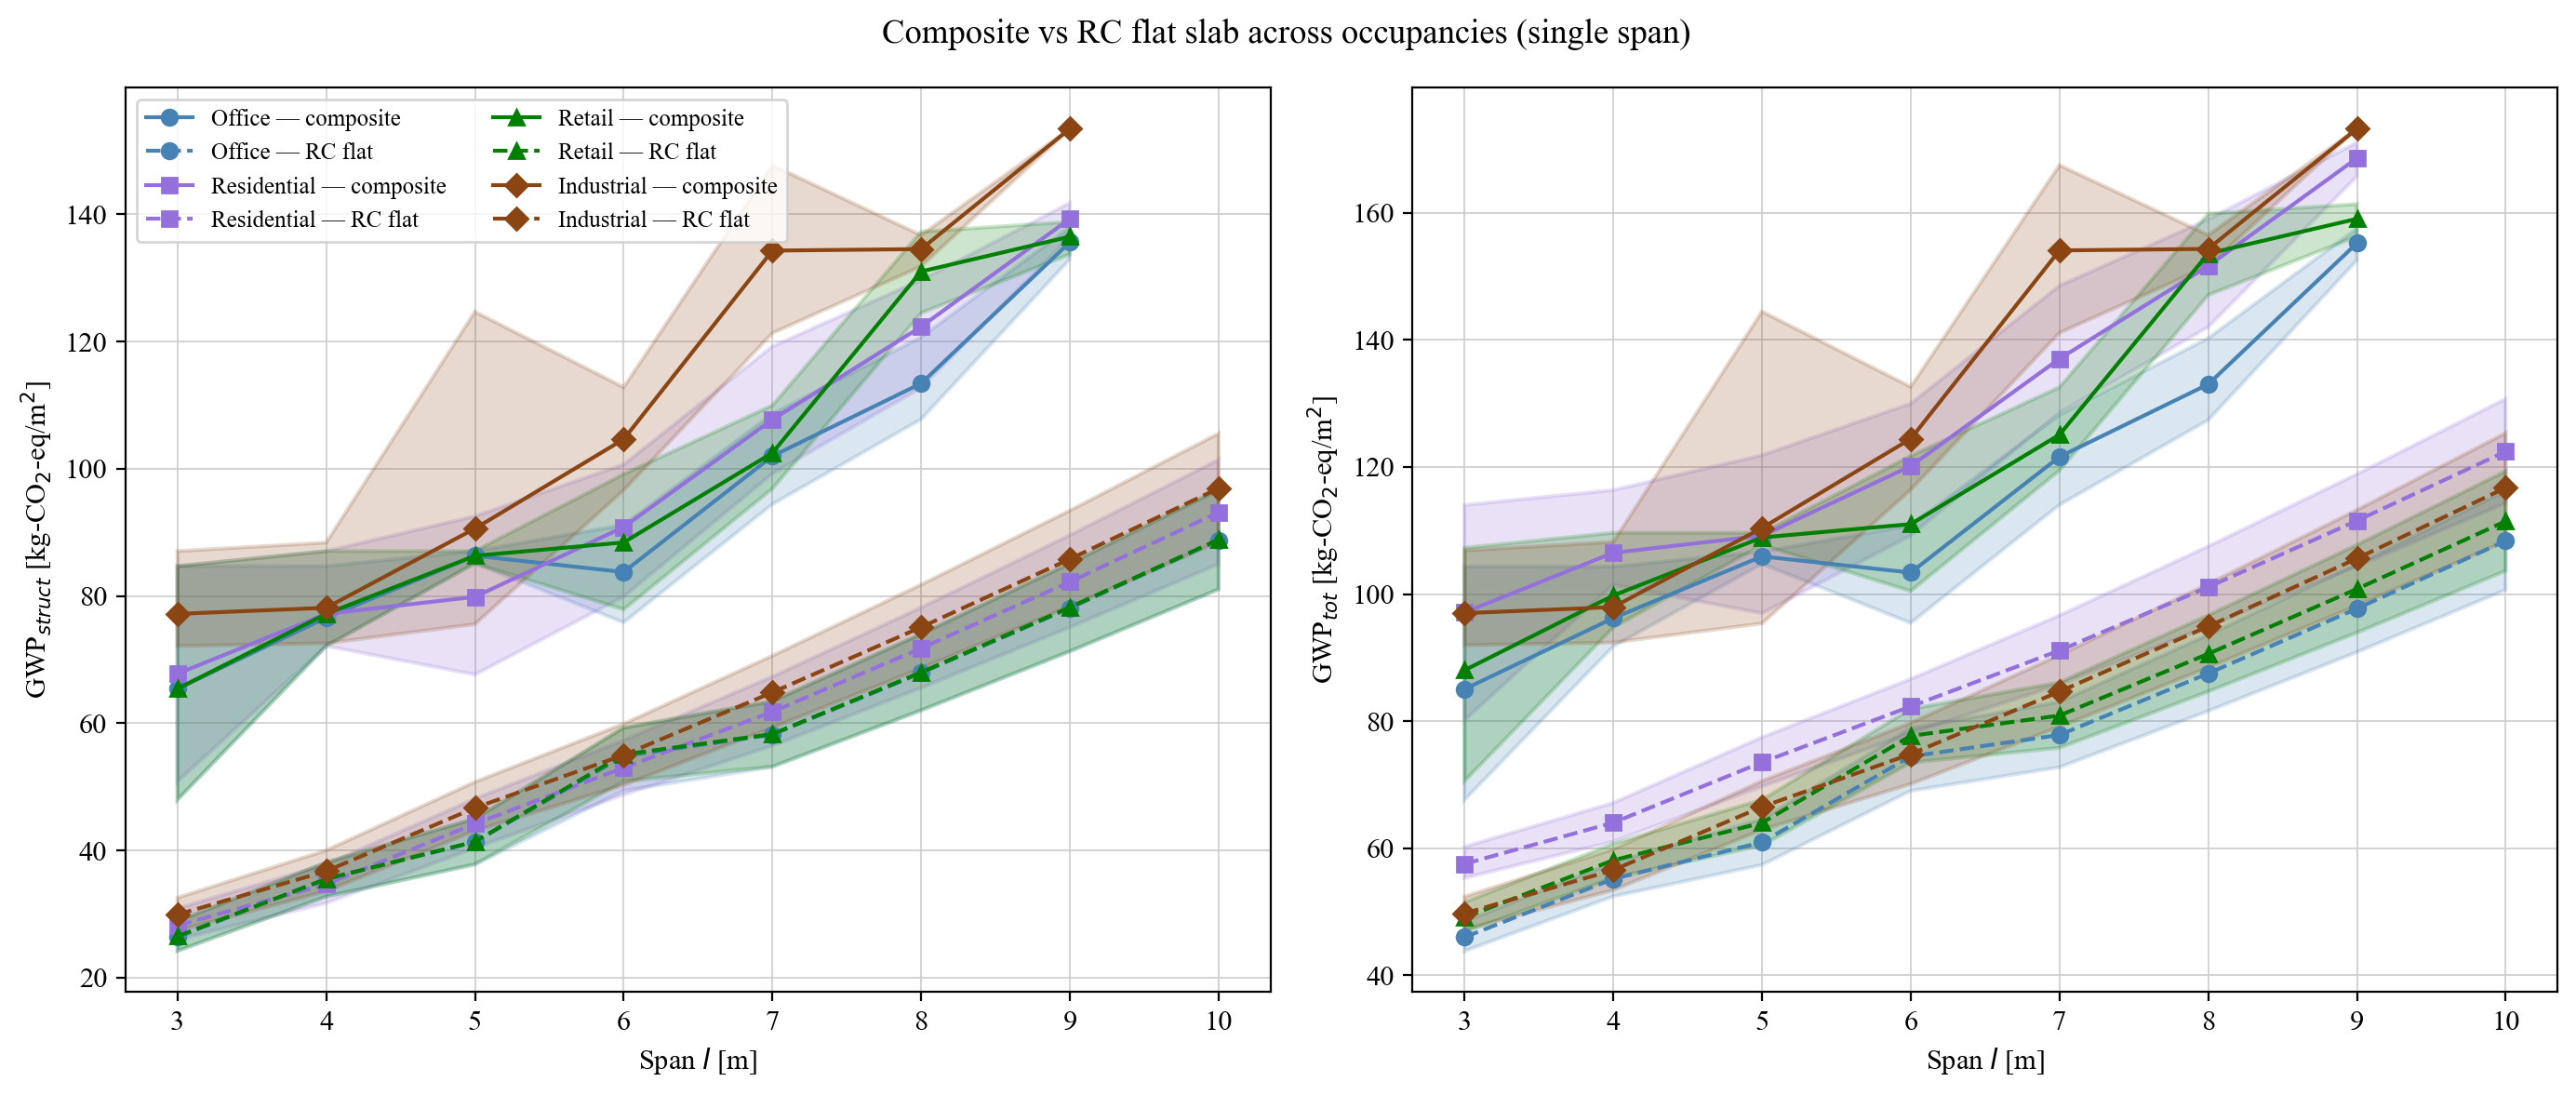
\includegraphics[width=0.9\textwidth]{figures/fig_composite_vs_rc_occupancies.png}
    \caption[Composite versus RC flat across occupancies]{Total GWP versus span for the composite slab (solid) and RC flat slab (dashed) in all four occupancy scenarios, single span.}
    \label{fig:cross_scenario}
\end{figure}

Across all four occupancies the composite slab is the highest--carbon system and the ranking of the five systems is preserved. The absolute GWP scales with imposed load and build--up mass (industrial highest, office lowest), but the \emph{relative} position of the composite slab does not change. The composite--to--RC--flat gap is narrowest for office (the lightest loading) and widest for industrial, indicating that the carbon disadvantage of composite construction grows with imposed load.

%==============================================================================
\subsection{Building-envelope comparison}
\label{sec:res_envelope}
%==============================================================================
The per-unit-area comparisons above treat each floor system in isolation. At the scale of a whole building, however, the structural depth of the floor has a further consequence: for a fixed overall building height, a shallower floor-to-floor construction depth allows more storeys to be accommodated, and hence more lettable or usable floor area. This building-envelope analysis translates the structural depth results into an achievable storey count, providing a building-level perspective that the per-square-metre GWP comparison does not capture.

For each slab system, span, and span configuration, the floor-to-floor height was computed as the sum of the clear storey height, the structural slab depth $h$ (the minimum-GWP section from the optimisation), and a fixed ceiling/services void. The achievable storey count is then the fixed building height divided by this floor-to-floor height. The building parameters assumed for each occupancy are typical values for that use: an office building of 40\,m with 2.7\,m clear height and a 0.40\,m services void; a residential building of 30\,m with 2.5\,m clear height and a 0.20\,m void; a retail building of 20\,m with 4.0\,m clear height and a 0.35\,m void; and an industrial building of 12\,m with 6.0\,m clear height and a 0.25\,m void. The resulting storey counts are continuous; the achievable integer count is the floor of each value. The results are tabulated in Table~\ref{tab:envelope_office_storey}.

\begin{table}[h!]
\centering
\small
\caption{Achievable storey count vs span --- Office (building height = 40\,m, clear height = 2.7\,m, ceiling void = 0.40\,m). Values are continuous; $\lfloor n \rfloor$ gives the achievable integer count.}
\label{tab:envelope_office_storey}
\begin{tabular}{lrrrrrrrr}
\toprule
Slab type & 3\,m & 4\,m & 5\,m & 6\,m & 7\,m & 8\,m & 9\,m & 10\,m \\
\midrule
Composite (SS) & 12.13 & 11.57 & 11.84 & 11.54 & 11.29 & 11.10 & 11.25 & --- \\
Composite (2-span) & 12.13 & 11.57 & 11.55 & 12.00 & 11.33 & 11.21 & --- & --- \\
Composite (3-span) & 12.13 & 11.57 & 11.58 & 11.98 & 11.44 & 11.30 & 11.19 & --- \\
\midrule
RC Solid & 12.26 & 12.06 & 12.05 & 11.87 & 11.84 & 11.71 & 11.59 & 11.45 \\
RC Ribbed & 11.95 & 11.67 & 11.53 & 11.41 & 11.21 & 11.11 & 10.91 & 10.79 \\
Timber Solid & 11.81 & 11.67 & 11.50 & 11.48 & 11.32 & 11.16 & 10.98 & 10.99 \\
Timber Ribbed & 11.21 & 11.21 & 11.12 & 11.05 & 10.82 & 10.49 & 10.29 & 10.07 \\
\bottomrule
\end{tabular}
\end{table}

\begin{figure}[h!]
    \centering
    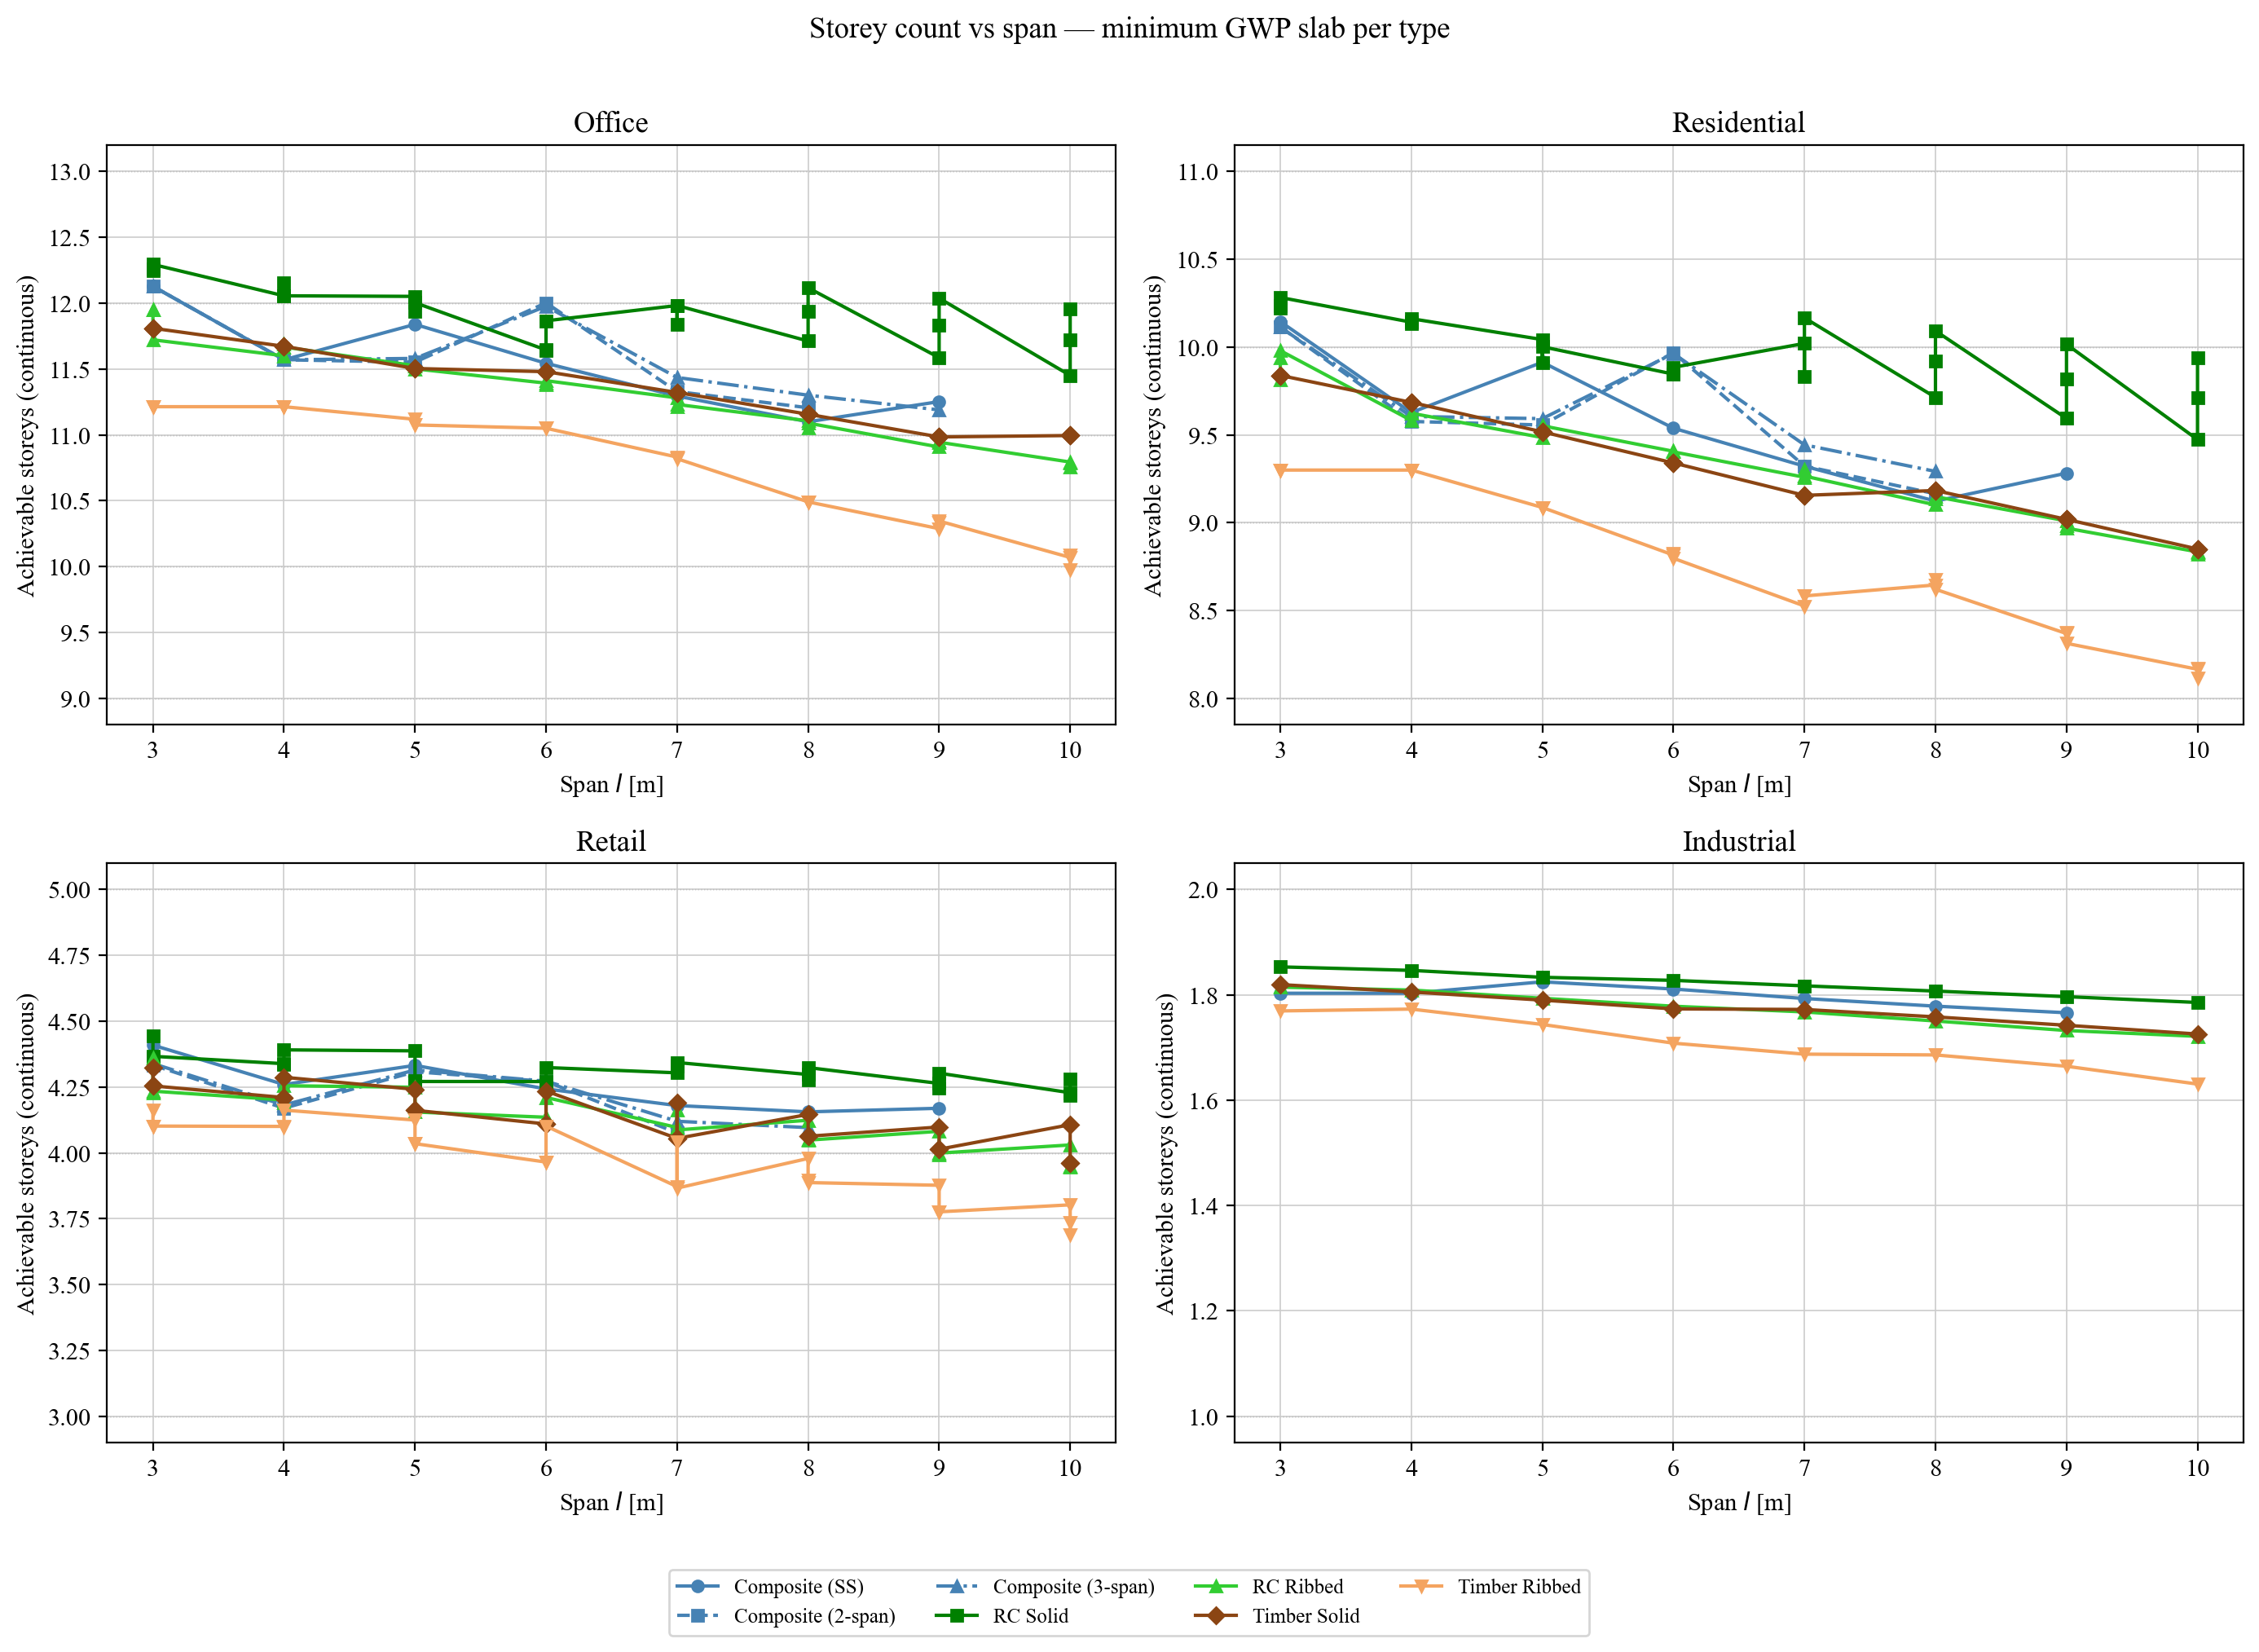
\includegraphics[width=\textwidth]{figures/fig_envelope_storey_count.png}
    \caption[Achievable storey count versus span, all occupancies]{Achievable storey count versus span for the minimum--GWP section of each slab system, across all four occupancy scenarios}
    \label{fig:envelope_storey_count}
\end{figure}

The building-envelope ranking differs markedly from---and is in large part the inverse of---the embodied-carbon ranking. The RC solid (flat) slab, being the shallowest structural section across almost the entire span range, achieves the highest storey count in every occupancy. The composite slab ranks second at short spans (for example 12.13 achievable storeys at 3\,m office, against 12.26 for RC solid) but falls back towards the middle at longer spans, where its deep-deck sections increase the floor-to-floor height. Critically, the two systems that performed best on embodied carbon---the timber rectangular and RC ribbed slabs---perform worst on storey count, because their greater structural depth consumes more of the building height per floor. The timber ribbed slab, with the deepest sections, achieves the fewest storeys throughout.

This result reframes the headline finding of this chapter. On embodied carbon alone the composite slab is the least favourable system (Section~\ref{sec:res_office_gwp}); on building-height efficiency it is among the best, second only to the RC flat slab and well ahead of the low-carbon timber and ribbed systems. The depth-competitiveness of the composite slab---its ability to deliver nearly as many storeys as the RC flat slab---is one of the practical advantages that offsets its higher embodied carbon, and is examined further in the discussion (Chapter~\ref{fifthchapter}).

%==============================================================================
\subsection{Validation against manufacturer tables}
\label{sec:res_validation}
%==============================================================================
To establish confidence in the structural model, the maximum permissible span computed by the optimiser for each deck was compared against the manufacturer's published load/span tables. For every deck profile and gauge for multispan decks, the model's design span was expressed as a ratio of the manufacturer's tabulated maximum span for the equivalent loading; a ratio at or below unity indicates that the model design lies within the manufacturer's envelope. Comparisons were made against both British Standard and Eurocode manufacturer tables as available, at an imposed load of 5 or 6\,kN/m$^2$ depending on the tables used.

Of the 406 deck--span--configuration combinations checked, 103 had no comparable manufacturer table (chiefly propped cases for which no propped table is published) and were excluded. Of the 303 comparable checks, 266 (87.8\,\%) passed, and---importantly---every passing case lies within the manufacturer envelope (span ratio $\leq 1.0$, mean 0.78). The model is therefore consistently conservative relative to the published tables. Table~\ref{tab:verification} summarises the outcome by deck family and Figure~\ref{fig:verification} shows the span-ratio distribution for every deck.

\begin{table}[h!]
\small\centering
\caption{Verification against manufacturer load/span tables, by deck family. ``Comparable'' excludes cases with no published table.}
\label{tab:verification}
\begin{tabular}{lcccc}
\toprule
Deck family & Comparable & Pass & Fail & Pass rate \\
\midrule
ComFlor 46  & 6   & 6   & 0  & 100\,\% \\
ComFlor 51  & 42  & 39  & 3  & 93\,\% \\
ComFlor 60  & 56  & 42  & 14 & 75\,\% \\
ComFlor 80  & 43  & 34  & 9  & 79\,\% \\
ComFlor 210 & 25  & 16  & 9  & 64\,\% \\
ComFlor 225 & 27  & 25  & 2  & 93\,\% \\
Multideck 60  & 33 & 33 & 0 & 100\,\% \\
Multideck 80  & 30 & 30 & 0 & 100\,\% \\
Multideck 146 & 41 & 41 & 0 & 100\,\% \\
\midrule
\textbf{Total} & \textbf{303} & \textbf{266} & \textbf{37} & \textbf{87.8\,\%} \\
\bottomrule
\end{tabular}
\end{table}

\begin{figure}[h!]
    \centering
    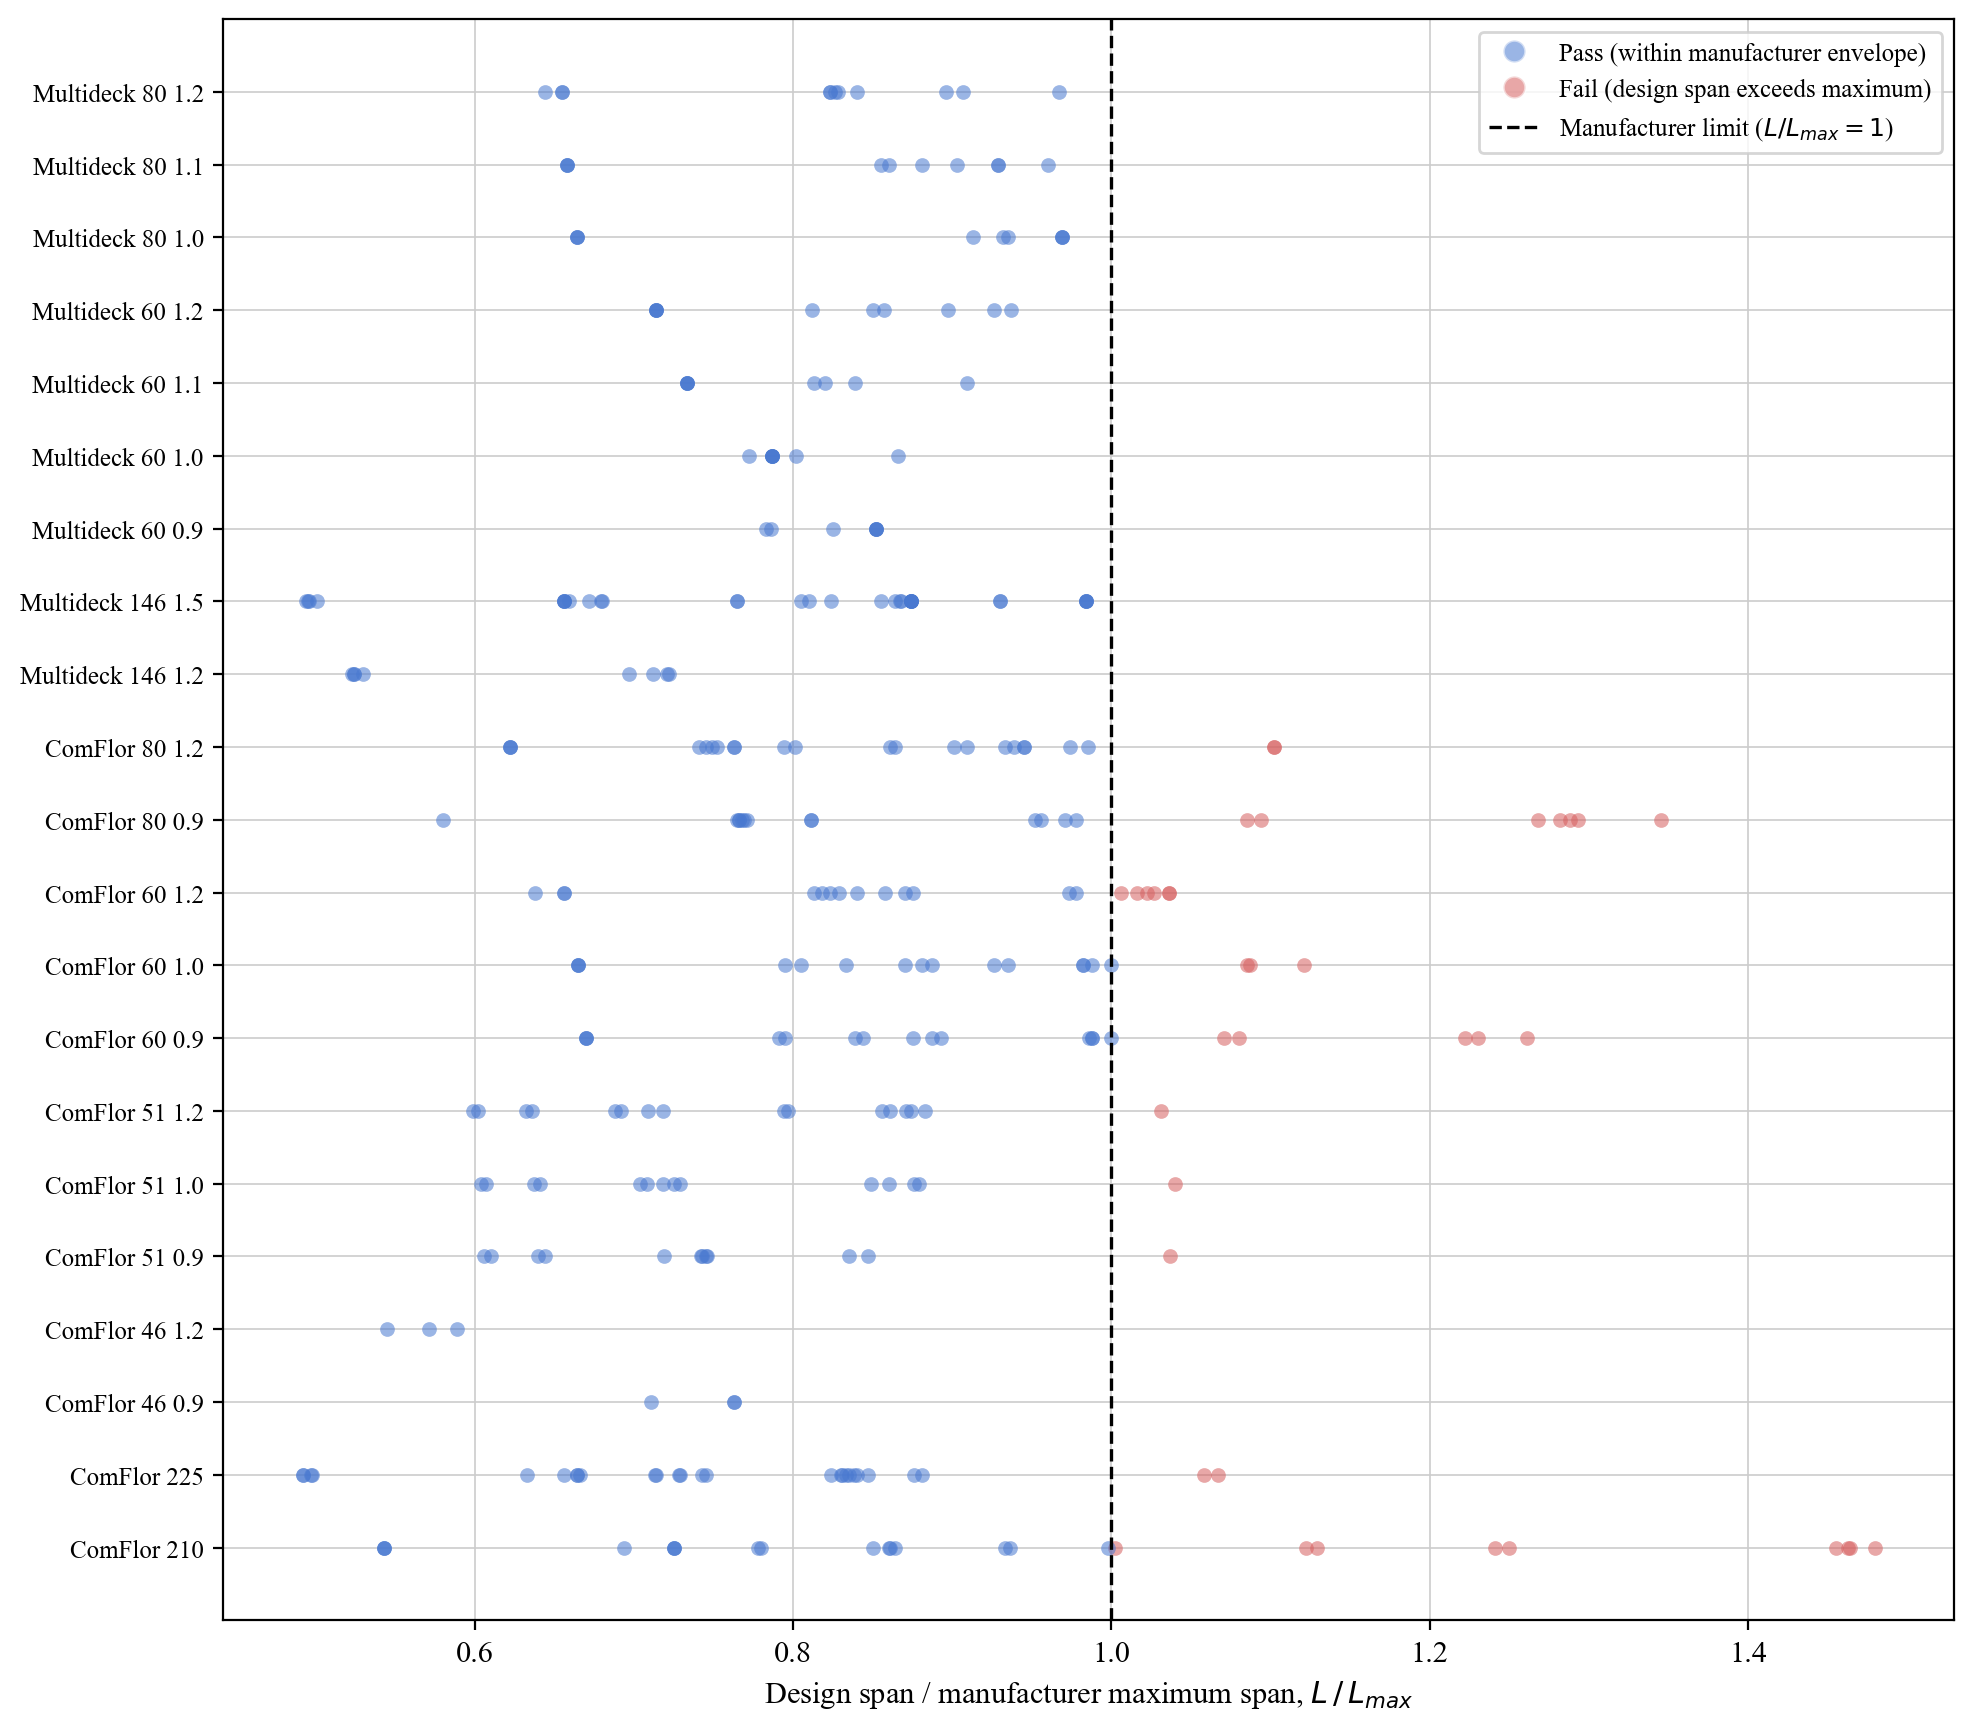
\includegraphics[width=0.95\textwidth]{figures/fig_mfr_verification.png}
    \caption[Model span versus manufacturer maximum]{Design span as a fraction of the manufacturer's published maximum span, for every deck profile and gauge.}
    \label{fig:verification}
\end{figure}

All 37 failures share two features: they are all propped cases, and all occur where the model's design span only marginally exceeds the manufacturer's tabulated maximum (span ratio just above unity, for example ComFlor 60 0.9 at 5\,m against a published maximum of 4.63\,m). They are concentrated in the deeper ComFlor profiles (210, 80, 60) at their longest spans, and are more frequent for the Eurocode-based tables (17\,\% fail) than the British Standard tables (7\,\%) and for the three-span configuration. The Multideck range passes without exception. Since these marginal cases sit at the limit of each deck's span range and the optimiser does not select them as GWP optima, the verification gives good confidence in the structural model across the span range relevant to the results.

%==============================================================================
\subsection{Summary}
\label{sec:res_summary}
%==============================================================================
The central result of this study is consistent across all four occupancy scenarios, all three span configurations, and the full practical span range: the composite steel--concrete slab carries the highest embodied carbon of the five floor systems compared, exceeding the RC flat baseline by a margin that widens with both span and imposed load, and exceeding the RC ribbed and timber systems by even larger margins. The composite design is governed by SLS deflection (single span) or by hogging at internal supports (continuous spans) over most of the range, with fire and longitudinal shear governing only at the shortest spans; it requires propped construction at spans over 5\,m for the office range and, under industrial loading, reaches at most 7\,m in both the two-- and three--span configurations. These findings answer the primary research question directly---on embodied carbon alone, the composite slab does not offer an advantage over reinforced concrete flat slabs---and motivate the discussion in Chapter~\ref{fifthchapter}, where the non--carbon considerations that nonetheless favour composite construction (construction speed, structural depth, service integration, and cost) are examined.
